\documentclass{IFNMG}


% =========================================================
% Adicione aqui os pacotes extras, caso necessário.
%
\usepackage{tasks, enumerate, diagbox, ulem, multicol, cancel}


% ===============================================
% Abreviação de Comandos e novos comandos
%
\theoremstyle{definition}
\newtheorem{teorema}{Teorema}[subsection]
\newtheorem{definicao}{Definição}[subsection]
\newtheorem{exemplo}{Exemplo}[subsection]
\newtheorem{observacao}{Observação}[subsection]
\newcommand{\N}{\mathbb{N}}
\newcommand{\Z}{\mathbb{Z}}
\newcommand{\Q}{\mathbb{Q}}
\newcommand{\R}{\mathbb{R}}
\newcommand{\C}{\mathbb{C}}

\newcommand{\F}{\mathbb{F}}
\newcommand{\md}{\text{mod  )}}

% =========================================================
% Hifenização de Palavras
%
\hyphenation{ci-vi-li-za-ções}


\begin{document}
% =========================================================
% INFORMAÇÕES SOBRE O TCC
%
\author{Isak Paulo de Andrade}{Ruas}
\title{Criptografia de curvas elípticas sobre corpos de Galois:}{um estudo de caso}
\orientador{Dr. Josué Antunes de Macêdo}
\coOrientador{}
\graduacao{Licenciatura}{Matemática}
\campus{Januária}{MG}
\date{Janeiro}{2022}


%%%% Banca Avaliadora
\avaliadorUm{Lílian Isabel Ferreira Amorim}
\avaliadorDois{Adriana Martins da Silva Castro}


% =========================================================
% ELEMENTOS PRÉ-TEXTUAIS
%
%\maketitle			% Cria Capa e Folha de Rosto
%
%\folhaDeAprovacao
%
%\listaDeFiguras
%\listaDeTabelas
%
%\dedicatoria
%\agradecimentos
%\epigrafe
%
%\resumo
%
%\sumario

% =========================================================
% ELEMENTOS TEXTUAIS
%%%%% Introdução
\section{INTRODUÇÃO}

Esta pesquisa foi motivada pela necessidade de entender a estrutura e
funcionamento da criptografia de ponta a ponta no contexto digital. Questões
como: \textit{"Como funciona a criptografia de ponta a ponta?"}, e
\textit{"Como podemos assegurar a autenticidade do remetente e a integridade da
	mensagem?"} serviram como base para o desenvolvimento deste estudo.

A criptografia é uma ferramenta indispensável na garantia da privacidade e
segurança das comunicações no mundo digital. No entanto, o desenvolvimento e
implementação de sistemas de criptografia eficientes e seguros ainda consiste
em um desafio para muitos desenvolvedores e organizações. Sistemas de
criptografia, como os baseados em curvas elípticas, possuem uma complexidade
matemática intrínseca que pode tornar seu entendimento e implementação um
processo complexo.

O objetivo desta pesquisa é desmistificar o funcionamento da criptografia
baseada em curvas elípticas e fornecer uma implementação passo a passo deste
sistema. Este estudo é relevante pois pode servir de guia para desenvolvedores
e pesquisadores que necessitam compreender a matemática por trás deste tipo de
criptografia e saber como aplicá-la em situações práticas.

Além disso, considerando o papel primordial da criptografia nos dias atuais
para a proteção de dados e garantia da privacidade no ambiente digital, este
trabalho também tem como propósito contribuir para a literatura na área de
segurança cibernética e criptografia. A pesquisa vai além de apenas apresentar
fundamentos teóricos, propondo também uma implementação prática que possa ser
facilmente reproduzida por outros profissionais da área.

A criptografia de curva elíptica tem se destacado como uma alternativa
eficiente em relação a outras técnicas, devido ao seu desempenho
consideravelmente superior com chaves de tamanho reduzido. Dessa forma, um
estudo aprofundado sobre o uso de curvas elípticas na criptografia traz uma
contribuição significativa tanto para a comunidade acadêmica quanto para a
indústria.

Finalmente, esta investigação parte de um questionamento genuíno e uma busca
por um entendimento técnico e prático dos conceitos que governam as aplicações
de segurança digital. A busca por respostas a estas perguntas possibilita uma
compreensão mais aprofundada dos sistemas criptográficos e permite uma análise
mais crítica do cenário atual da segurança de dados.
%
%%%%%% Revisão da Literatura
\newpage
% **
% Revisão da literatura.
% *

\section{PANORAMA HISTÓRICO DA CRIPTOGRAFIA}

A criptografia é uma ferramenta indispensável para a proteção de informações.
Derivada do grego "kriptos", que significa "secreto", e "graphia", que se
refere à "escrita", é uma ferramenta indispensável para a proteção de
informações (Pabón Cadavid, 2010, p. 59) ou (Filho e Azeredo, 2017, p. 23).
Envolve a utilização de algoritmos para transformar a informação original em um
formato indetectável e inacessível a indivíduos sem autorização. Ela desempenha
um papel crucial na garantia da segurança da transmissão de informações,
especialmente em redes ou ambientes considerados inseguros (Viana \textit{et
	al}, 2022, p. 226).

Com sua origem na antiguidade, a criptografia já era utilizada em situações
militares complexas, conforme relatados Heródoto; destacou-se ainda mais
sobre figuras históricas como Júlio César, que utilizou técnicas
esteganográficas e criptográficas em suas comunicações para garantir a
confidencialidade das informações. A introdução dos sistemas elétricos de
transmissão de informações impulsionou a criptografia para uma
nova trajetória, tornando-se o precursora do que conhecemos hoje (Pabón
Cadavid, 2010, p. 61-63).

\subsection{Origem e desenvolvimento da criptografia}

A era moderna, especialmente após a Segunda Guerra Mundial, trouxe avanços
tecnológicos notáveis na criptografia. Durante esse período, houve uma expansão
significativa na pesquisa e desenvolvimento em criptografia, o que despertou
não apenas o interesse das forças armadas e dos governos, mas também do público
em geral. Com o crescimento da pesquisa e do desenvolvimento no campo, houve a
criação de sistemas computacionais avançados para fins de criptografia,
destacando-se como ferramentas essenciais para a segurança da informação (Pabón
Cadavid, 2010, p. 64).

Neste cenário, grandes descobertas, como a máquina de Charles Babbage e as
bombas de Turing de Alan Turing, desempenharam um papel crucial. Essas
invenções, originalmente voltadas para o desciframento de códigos, se tornaram
fundamentais para o desenvolvimento da tecnologia informática atual. É
importante ressaltar que sem esses desenvolvimentos pioneiros na criptografia,
a revolução da tecnologia da informação poderia ter tomado um curso bastante
diferente, evidenciando o papel crucial da criptografia na evolução da
tecnologia (Pabón Cadavid, 2010, p. 64).

A criptografia moderna, embora mantenha a essência de sua prática histórica, se
tornou amplamente complexa devido ao avanço tecnológico. Sua execução não se
limita mais à simples reorganização do alfabeto, mas incorpora algoritmos
matemáticos complicados para cifrar mensagens. Da mesma forma, a tarefa de
"quebrar" códigos criptográficos, a criptoanálise, sai da capacidade humana de
observar padrões de repetição de letras, tornando-se dependente da potência de
supercomputadores. Dessa forma, se torna quase impossível criar códigos seguros
e descriptografá-los sem um sólido conhecimento em matemática, considerável
poder de processamento de dados e um substancial investimento financeiro
(Abreu, 2017, p. 28)

\subsection{Adaptação da criptografia ao mundo moderno}

No mundo contemporâneo, cada vez mais imerso em digitalização e conectividade,
não podemos ignorar a preponderância e a importância vital da criptografia. Há
uma presença profunda e abrangente da tecnologia em nossas vidas cotidianas,
desde comunicação pessoal, transações financeiras até a infraestrutura crucial
de qualquer nação. Tudo isso cria um cenário onde a segurança dos dados online
se torna não apenas desejável, mas uma absoluta necessidade.

Nesse cenário, a criptografia emerge como um componente soberano na garantia da
segurança e privacidade do usuário na internet. Este foco elevado na
criptografia é compreensível considerando que ela proporciona um canal seguro
para troca de informações delicadas nesse mar aberto e incerto que é a web
(Viana \textit{et al}, 2022, p. 231-236). A criptografia não apenas permeia o
tecido de nossas interações online como indivíduos, mas também desempenha um
papel crucial para entidades empresariais e governamentais. Seu alcance não se
restringe somente a aplicativos e websites; na verdade, ela é de vital
importância para sistemas mais complexos e intrincados.

É nesses sistemas que evidenciamos sua relevância no setor privado. As trocas de
informações confidenciais são recorrentes nas interações empresariais, e a
criptografia se torna um escudo protetor, guardião da integridade dessas
informações. Além disso, situações de hostilidade, como períodos de guerra ou
conflito, reforçam ainda mais a necessidade de mensagens codificadas para garantir
a segurança e evitar deturpações (Andria; Gondim; Salomão, 2019, p. 31-36).
Por outro lado, as transações financeiras se tornaram primariamente digitais devido
ao conveniente avanço tecnológico. Essa transição para o meio digital das
transações financeiras, junto com atividades comerciais e assuntos corporativos
sensíveis, certamente exigem um nível de confidencialidade que somente a criptografia
pode providenciar adequadamente.

Cada dia mais pessoas estão se deliciando com a comodidade que a internet
proporciona, sem se dar conta de que cada transação, cada troca de dados
seguros, é facilitada e resguardada por diversos sistemas de criptografia que
trabalham incansavelmente em segundo plano. Por esse motivo, podemos afirmar
sem hesitação que a criptografia não é apenas um luxo, mas uma necessidade
crucial que proporciona a segurança e confiança tão necessárias na atual era
digital (Andria; Gondim; Salomão, 2019, p. 31-36). Com tudo isso em mente,
fica claro que sem a presença vital da criptografia, o ciberespaço atual seria
um lugar muito mais perigoso e imprevisível de se navegar.

\subsection{Os impasses legais na utilização da criptografia}

Na era da economia digital avançada e da transformação digital disseminada na
vida cotidiana, a demanda por sistemas seguros e confiáveis está em progressivo
crescimento. Ao atender essas demandas, a criptografia emerge como uma
protagonista estratégica. Ela atua como uma poderosa ferramenta na salvaguarda
de dados, assegurando que as informações transmitidas permaneçam inacessíveis a
olhares indesejados (Viana \textit{et al}, 2022, p. 231-232). No entanto,
lançamos nosso olhar a um peculiar dilema quando o 'olhar indesejado' que tenta
acessar essas informações se identifica como o próprio Estado.

A capacidade da criptografia em manter os dados impenetráveis e invioláveis
frequentemente se torna o núcleo dos debates legais entre as grandes empresas
tecnológicas e os governos. Estas discussões centram-se na dificuldade ou, em
muitos casos, na impossibilidade de se violar a privacidade que esses sistemas
criptográficos garantem. Podemos observar esse conflito através de casos
emblemáticos, como o do aplicativo de mensagens instantâneas WhatsApp,
bloqueado três vezes no Brasil por se recusar a fornecer o conteúdo de
comunicações dos investigados em processos criminais (Abreu, 2017, p. 28).

Seguindo essa mesma linha, podemos revisitar o conflito de 2015 entre a Apple e
o governo dos EUA. A face a face de discordâncias aconteceu por causa dos
robustos mecanismos de criptografia utilizados nos iPhone, considerados
invioláveis pelo governo. Este evento sublinha a tensão inerente na relação
entre os Estados e a criptografia: é uma ferramenta que uso, mas rejeito seu
uso por outros, especialmente quando esses "outros" são considerados potenciais
adversários (Abreu, 2017, p. 28). Essa dualidade mostra a complexidade da
relação entre segurança, privacidade e governança na era digital.

\subsection{Criptografia: um olhar para o futuro}

Portanto, a importância da criptografia não é uma questão só do passado ou do
presente. Sua relevância se perpetua ao longo do tempo, evoluindo constante e
adaptativamente para atender necessidades emergentes de segurança e para
sustentar a confiabilidade na digitalização crescente (Viana \textit{et al},
2022, p. 234). A habilidade de cifrar mensagens, permitindo uma comunicação
segura e privada, volta-se cada vez mais indispensável em uma sociedade que é,
ao mesmo tempo, altamente digital e globalmente interconectada.

A criptografia, cujo papel tem sido de relevância para a humanidade desde os
tempos antigos, certamente continuará a ser uma peça chave no nosso futuro
digital. Por garantir a privacidade e a segurança das informações, a
criptografia é uma ferramenta crucial para proteger dados em um mundo que se
torna cada dia mais dependente da tecnologia e da digitalização. Sua
relevância, longe de diminuir, só tem a crescer e se adaptar para atender às
novas demandas e necessidades de segurança que irão surgir.

\section{FUNDAMENTOS E CARACTERÍSTICAS DA CRIPTOGRAFIA}

\subsection{Entendendo a criptografia simétrica}

\begin{figure}[h!] \centering
	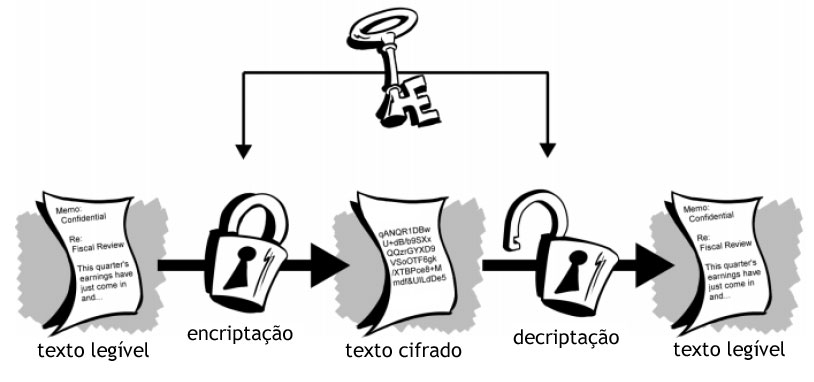
\includegraphics[width=0.7\textwidth]{Imagens/ilustracao_do_processo_de_criptografia_simetrico}
	\caption{Ilustração do processo de criptografia Simétrico}
	Fonte: Seragiotto, 2023, p. ?
\end{figure}

A criptografia simétrica, de processo ilustrado na Figura 1, é um dos
principais métodos de criptografia, onde é usada uma única chave tanto para
criptografar quanto para descriptografar os dados. Este sistema é eficiente e
rápido, onde o remetente utiliza a chave para transformar a mensagem em um
formato ilegível, sendo então revertida no lado do destinatário usando a mesma
chave (Viana \textit{et al}, 2022, p. 235-236)

\begin{CitacaoLonga}
	Essencialmente, quando a origem (ALFA) cifra uma mensagem, ele utiliza um
	algoritmo de ciframento para transformar o conteúdo em claro da mensagem em
	texto cifrado. Quando o destino (BRAVO) decifra uma mensagem, ele utiliza o
	algoritmo de deciframento correspondente para converter o texto cifrado de novo
	em uma mensagem clara. Se um intruso (CHARLIE) conhecer o algoritmo de
	ciframento, ele poderia decifrar uma mensagem cifrada tão facilmente quanto o
	destino (BRAVO). A solução no uso da criptografia de chave privada propõe que
	quando a origem (ALFA) cifra uma mensagem, ele utilize um algoritmo de
	ciframento e uma chave secreta para transformar uma mensagem clara em um texto
	cifrado. O destino (BRAVO), por sua vez, ao decifrar a mensagem, utiliza o
	algoritmo de deciframento correspondente e a mesma chave para transformar o
	texto cifrado em uma mensagem em claro. O intruso (CHARLIE), por não possuir a
	chave secreta, mesmo conhecendo o algoritmo, não conseguirá decifrar a
	mensagem. A segurança do sistema passa a residir não mais no algoritmo e sim na
	chave empregada. É ela (chave privada) que agora, no lugar do algoritmo, deverá
	ser mantida em segredo pela origem (ALFA) e destino (BRAVO) (Oliveira, 2012, p. 3)
\end{CitacaoLonga}

Entretanto, um desafio crítico ao utilizar esse sistema é o compartilhamento
seguro da chave que deve ser efetuado entre o remetente e o destinatário. Este
processo precisa ser seguro para evitar que indivíduos mal-intencionados
interceptem a chave e tenham acesso à informação enviada (Viana \textit{et al},
2022, p. 236)

\subsection{Entendendo a criptografia assimétrica}

\begin{figure}[h!] \centering
	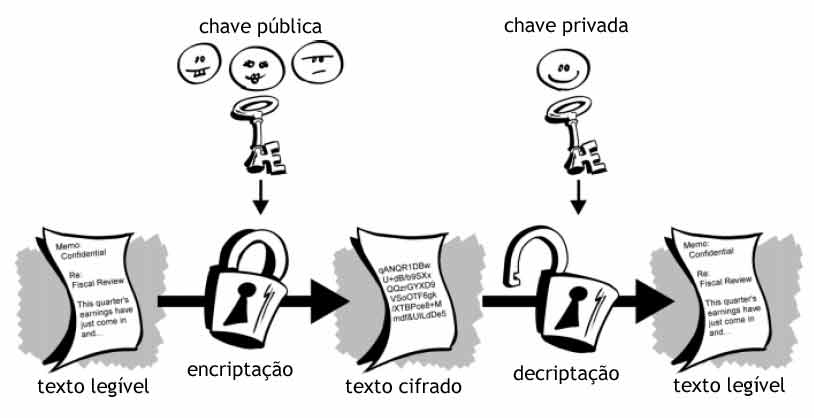
\includegraphics[width=0.7\textwidth]{Imagens/ilustracao_do_processo_de_criptografia_assimetrico}
	\caption{Ilustração do processo de criptografia Assimétrico}
	Fonte: Seragiotto, 2023, p. ?
\end{figure}

Contrastando com a criptografia simétrica, temos a criptografia assimétrica, de
processo ilustrado na Figura 2, também conhecida como criptografia de chave
pública. Aqui, um par de chaves é usado, sendo elas a chave pública, que pode
ser compartilhada abertamente, e uma chave privada, que deve ser mantida em
sigilo somente pelo destinatário da mensagem (Viana \textit{et al}, 2022, p.
238)

\begin{CitacaoLonga}
	Essencialmente, o destino (BRAVO) e todos os que desejam comunicar-se de modo
	seguro geram uma chave de ciframento e sua correspondente chave de
	deciframento. Ele mantém secreta a chave de deciframento, esta é chamada de sua
	chave privada. Ele torna pública a chave de ciframento, esta é chamada de sua
	chave pública. A chave pública realmente condiz com seu nome. Qualquer pessoa
	pode obter uma cópia dela. O destino (BRAVO) inclusive encoraja isto,
	enviando-a para seus amigos ou publicando-a na internet. Assim, O intruso
	(CHARLIE) não tem nenhuma dificuldade em obtê-la. Quando a origem (ALFA) deseja
	enviar uma mensagem ao destino (BRAVO), precisa primeiro encontrar a chave
	pública dele. Feito isto, ela cifra sua mensagem utilizando a chave pública do
	destino (BRAVO), despachando-a em seguida. Quando o destino (BRAVO) recebe a
	mensagem, ele a decifra facilmente com sua chave privada. O intruso (CHARLIE),
	que interceptou a mensagem em trânsito, não conhece a chave privada do destino
	(BRAVO), embora conheça sua chave pública. Mas este conhecimento não o ajuda a
	decifrar a mensagem. Mesmo a origem (ALFA), que foi quem cifrou a mensagem com
	a chave pública do destino (BRAVO), não pode decifrá-la agora. (Oliveira, 2012,
	p. 4)
\end{CitacaoLonga}

Para enviar uma mensagem utilizando criptografia assimétrica, a chave pública
do destinatário é usada pelo remetente para criptografar a mensagem. Esta só
pode ser decriptada e lida pelo destinatário que possui a chave privada
correspondente. Isso adiciona uma camada extra de segurança à mensagem, pois a
chave privada é exclusiva do destinatário (Viana \textit{et al}, 2022, p. 240)

\subsection{Contrapontos entre criptografia simétrica e assimétrica}

A criptografia simétrica e a criptografia assimétrica possuem diferenças
essenciais que ditam suas aplicações ideais. A criptografia simétrica é rápida
e eficiente, tornando-a ideal para a codificação de conteúdos de mensagens.
Isso garante a confidencialidade de dados no processo de transmissão. No
entanto, as abordagens simétricas encontram suas principais desvantagens na
complexidade do gerenciamento e distribuição de chaves (Oliveira, 2012, p. 8).

Gerenciar e distribuir chaves é um desafio na criptografia simétrica, pois
exige um canal seguro para o compartilhamento das chaves entre emissor e
receptor. Esse processo se torna complicado, especialmente quando há um grande
número de participantes na transmissão de dados. Isso torna a gerência das
chaves extremamente difícil e vulnerável a falhas (Oliveira, 2012, p. 8).

Em contrapartida, a criptografia assimétrica resolve os problemas de
gerenciamento e distribuição de chaves que são inerentes à criptografia
simétrica. Embora seja mais lenta devido ao seu alto grau de complexidade, ela
fornece um nível maior de segurança. Isso ocorre através da separação das
chaves em públicas e privadas (Oliveira, 2012, p. 8).

Na criptografia assimétrica, a chave pública pode ser distribuída livremente.
Enquanto isso, a chave privada, utilizada para decodificar o documento
codificado, é conhecida apenas pelo seu proprietário. Além disso, este tipo de
criptografia é ideal para a distribuição de chaves e para assinatura digital.
Isso garante não apenas a confidencialidade, mas também a autenticidade e a
integridade das mensagens (Oliveira, 2012, p. 8).

% \begin{table}[h!]\centering
% 	\caption{Quadro comparativo}
% 	\begin{tabular}{ p{7.3cm} |  p{7.3cm}}
% 		\hline
% 		\textbf{Criptografia simétrica ou chave privada} & \textbf{Criptografia assimétrica ou chave pública} \\
% 		\hline
% 		Rápida                                           & Lenta                                              \\
% 		\hline
% 		Gerência e distribuição das chaves é complexa    & Gerência e distribuição das chaves é simples       \\
% 		\hline
% 		Não oferece assinatura digital                   & Oferece assinatura digital                         \\
% 		\hline
% 	\end{tabular}
% 	%
% 	\vspace*{0.4cm}\\ % Não apagar esta linha
% 	Fonte:  Oliveira, 2012,  p. 8
% \end{table}

% A Tabela 1 sumariza as características principais de cada abordagem da
% criptografia. Nota-se que a criptografia simétrica, apesar de ser mais rápida,
% é mais complexa em relação à gerência e distribuição de chaves e não oferece a
% funcionalidade de assinatura digital. Por contrapartida, a criptografia
% assimétrica, ainda que seja mais lenta, apresenta simplicidade no manejo e
% distribuição de chaves e proporciona a ferramenta de assinatura digital.

Ambas os sistemas de criptografia possuem suas vantagens e desvantagens.
Enquanto a criptografia simétrica é rápida e eficiente, a segurança do
compartilhamento de chaves é um desafio. Por outro lado, a criptografia
assimétrica fornece uma segurança extra com a separação de chaves em pública e
privada, mas pode ser mais lenta devido ao seu maior nível de complexidade. A
escolha do tipo de criptografia a ser usado depende das necessidades
específicas de segurança de cada situação.

%
%%%%%% Metodologia
\newpage
% **
% Metodologia.
% *
\section{METODOLOGIA}

A metodologia desta pesquisa foi estruturada em quatro etapas distintas:

Na primeira etapa, realizou-se uma revisão bibliográfica abrangente, na qual se
analisaram e interpretaram trabalhos científicos, monografias, teses,
dissertações e normas de instituições renomadas, como o National Institute of
Standards and Technology (NIST) dos EUA. O foco principal dessa revisão foi a
investigação da criptografia de ponta a ponta, curvas elípticas, corpos finitos
e os fundamentos matemáticos dos algoritmos de criptografia. Essa revisão
bibliográfica proporcionou uma sólida base teórica para o desenvolvimento das
etapas subsequentes do projeto.

Na segunda etapa, exploraram-se as propriedades dos algoritmos de criptografia
de ponta a ponta, com um enfoque particular naqueles baseados em curvas
elípticas. A análise concentrou-se em questões como a codificação e
decodificação de mensagens, o estabelecimento de chaves seguras, a troca de
informações e a assinatura digital. Essa análise teórica permitiu uma
compreensão mais aprofundada das características e dos desafios associados à
criptografia.

A terceira etapa envolveu o desenvolvimento de um \textit{software} simulador,
utilizando a linguagem de programação Python como plataforma de implementação.
A escolha do Python deveu-se à sua robustez e acessibilidade em temas de
segurança da informação e criptografia. Essa etapa transformou a teoria em
prática, permitindo a criação de um ambiente de simulação para os algoritmos de
criptografia estudados.

A quarta etapa contemplou a análise dos resultados gerados pelo
\textit{software} implementado. Realizaram-se testes de eficácia, eficiência e
confiabilidade dos algoritmos e protocolos utilizados. Durante essa fase,
observações e limitações identificadas nos testes foram cuidadosamente
documentadas e analisadas. Essa avaliação experimental forneceu insights
valiosos sobre o desempenho dos algoritmos em um ambiente prático.

%
%%%%%% Resultados e Discussões
%\newpage
%% **
% Resultados e discussões.
% *
\section{CRIPTOGRAFIA COM CURVAS ELÍPTICAS}

\subsection{Conceitos preliminares}

Neste trabalho, adotaremos como definição equação de Weierstrass simplificada
de uma curva elíptica sobre um corpo $\K$, resultado apresentado por Gonzaga e
Pesco (2021, p. 37), $i.e$

\begin{definicao}
	Uma curva elíptica $E  = \{(x, y) \in \K | (y^2 = x^3 + Ax + B)\}$ no qual $(car(\K) \notin \{2,3\})$
	e ($4A^3 +27B^2 \neq 0)$.
\end{definicao}

$4A^3 +27B^2 \neq 0$ é a condição necessária para que qualquer ponto $P \in E$ possua uma reta tangente
(seja diferenciável) e $car(\K) \notin \{2,3\}$ garante que haja inverso multiplicativo de $2$ e $3$ em
$\K$. Para uma implementação computacional mais eficiente (Gonzaga e Pesco, 2021, p. 43), adotaremos $\K$ como o corpo
dos inteiros módulo $p$, ou seja, adotaremos $\K = \Z_{p}$, desta forma, a definição anterior poderá ser
escrita como $E(\Z_{p}): y^2 \equiv x^3 + Ax + B \pmod{p}$, donde $4A^3 +27B^2 \neq 0 \pmod{p}$ (Andria; Gondim; Salomão, 2019, p. 82)
De maneira geral, é valida a proposição a seguir:

\begin{proposicao}
	Considere a curva elíptica $E$. O conjunto de pontos na curva sobre um corpo finito $\F_{p}$,
	$E(\F_{p})$, é um grupo abeliano finito.
\end{proposicao}

\begin{proof}
	Pode ser vista em Brady, Davis e Tracy (2010, p. 6-7).
\end{proof}

\begin{exemplo} \label{exemplo:cf947430-c71a-43f2-893a-13b1cd929605}
	Seja $E$ uma curva elíptica sobre $(\Z_{7}, \oplus)$ de equação $y^2 = x^3 + x + 1$, determine todos
	os pontos desta curva.
\end{exemplo}

Para encontrar a solução deste exemplo, podemos empregar a seguinte estratégia:
criaremos uma tabela para calcular os valores de $x$ e $y$ separadamente e, em
seguida, para cada valor de $x \in \Z_{7}$ , verificaremos se o resultado da
expressão $x^3 + x + 1$ é um quadrado perfeito. As tabelas a seguir apresentam
os resultados dessas operações:

\begin{table}[h!]\centering
	\caption{Lado esquerdo da equação $y^2 = x^3 + x + 1$: atribuindo valores à variável y}
	\begin{tabular}{|c|c|c|c|c|c|c|c|c|}
		\hline
		$y$   & 0 & 1 & 2 & 3 & 4  & 5  & 6  \\
		\hline
		$y^2$ & 0 & 1 & 4 & 2 & 2 & 4 & 1 \\
		\hline
	\end{tabular}
	\vspace*{0.4cm}\\ % Não apagar esta linha
	Fonte:  ----
\end{table}

\begin{table}[h!]\centering
	\caption{Lado direito da equação $y^2 = x^3 + x + 1$: atribuindo valores à variável x}
	\begin{tabular}{|c|c|c|c|c|c|c|c|}
		\hline
		$x$           & 0 & 1 & 2 & 3 & 4 & 5 & 6 \\
		\hline
		$x^3 + x + 1$ & 1 & 3 & 4 & 3 & 6 & 5 & 6 \\
		\hline
	\end{tabular}
	\vspace*{0.4cm}\\ % Não apagar esta linha
	Fonte:  ----
\end{table}

Deste modo, substituindo $x = 0$ no polinômio, obtemos $1$, observando-se a
coluna $y^2$, temos que $y = 1$ e $y = 6$ geram $y^2 =1$, assim, temos que os
pares ordenados formados são $(\overline{0}, \overline{1})$ e $(\overline{0},
	\overline{6})$. Realizando este procedimento para todas os valores de $x$,
encontramos: $E(\Z_{7}) = \{\mathcal{O}, (\overline{0}, \overline{1}),
	(\overline{0}, \overline{6}), (\overline{2}, \overline{2}), (\overline{2},
	\overline{5}) \}$. $\mathcal{O}$ é o elemento neutro de $(\Z_{7}, \oplus)$,
este ponto também conhecido como \textit{"ponto no infinito"}, sua existência é
garantida pelo Teorema \ref{teorema:6f3c8fca-7ceb-4797-830b-4af48c390972}.

\begin{teorema}\label{teorema:6f3c8fca-7ceb-4797-830b-4af48c390972}
	A curva elíptica $E$, com a estrutura de soma $\oplus$, é um grupo abeliano cujo elemento neutro é  $\mathcal{O}$.
\end{teorema}

\begin{proof}
	Pode ser vista em Silva, Salomão e Neves (2019, p. 85).
\end{proof}

Nesta sessão, apresentou-se os conceitos preliminares fundamentais para
compreensão das curvas elípticas, no qual observou-se sua lei de formação e o
método a ser empregado para se determinar os pontos da curva em $\Z_{p}$, na
próxima seção apresentaremos o método a ser utilizado para construir a tabua de
operação de $(\Z_{p}, \oplus)$.

\subsection{Algoritmo para adição de pontos em curvas elípticas}

\begin{teorema}\label{teorema:4d1e8442-1093-47f1-99d2-4b4f3c7f0b58}

	(Algoritmo Euclidiano Estendido - Lema de Bézout) Sejam $a$ e $b$ inteiros positivos.
	Então a equação nas variáveis $X$ e $Y$:
	\begin{equation} \label{equation:de2e5ccc-7b0a-4e0a-a9bd-9c6eb48e83c1}
		aX + bY = mdc(a, b)
	\end{equation}

	\justify
	Possui soluções inteiras, digamos $X = u_0$ e $Y = v_0$. Além disso, todas as
	suas soluções são da forma:
	\begin{equation}
		X = u_0 + \frac{bk}{mdc(a, b)} \label{equation:446a68d6-401a-4e3a-abd9-2cd8ff56c1d5}
	\end{equation}
	\begin{equation}
		Y = v_0 - \frac{ak}{mdc(a, b)} \label{equation:4077b258-6707-47ca-9bd9-41b5a5d3ed88}
	\end{equation}

	\justify
	com $k \in \Z$.

\end{teorema}

\begin{proof}
	Pode ser vista em Silva, Salomão e Neves (2019, p. 12-13).
\end{proof}

\begin{definicao} \label{definicao:38fb565b-5356-485a-bc23-f1d31dcd0f8f}
	Dado uma curva elíptica $E$ definida sobre $(\Z_p, \oplus)$ e os pontos $P =
		(x_1, y_1)$ e $Q = (x_2, y_2) \in E$, a soma $P \oplus Q$ resulta em $R = (x_3,
		y_3) \in E$ (consulte o Teorema
	\ref{teorema:6f3c8fca-7ceb-4797-830b-4af48c390972}). A operação $\oplus$ em $E$
	é definida da seguinte maneira:

	Se $P = Q$, calculamos o valor de $\lambda$ da seguinte forma:
	\begin{equation}
		\lambda = \frac{3x_1^2 + A}{2y_1} \pmod{p} \label{equation:6c395b0c-263e-48b1-bb81-69e261534d1b}
	\end{equation}

	Se $P \neq Q$, o valor de $\lambda$ é calculado como:

	\begin{equation}
		\lambda = \frac{y_2 - y_1}{x_2 - x_1} \pmod{p} \label{equation:a3d20958-5111-4874-9793-b9a714f013aa}
	\end{equation}

	Com base no valor de $\lambda$, determinamos as coordenadas do ponto $R$ como
	segue:

	\begin{equation}
		x_3 = \lambda^2 - x_1 - x_2 \pmod{p} \label{equation:da9ad657-8ab7-421d-a202-0cf463d28920}
	\end{equation}

	\begin{equation}
		y_3 = \lambda(x_1 - x_3) - y_1 \pmod{p} \label{equation:8c03bda8-df85-4e46-97f5-18acd9cb0a31}
	\end{equation}

\end{definicao}

\begin{exemplo} \label{exemplo:4508c716-b529-4e3d-aa71-9a4493c9b4a7}

	Considere a curva elíptica $E$ definida sobre $(\Z_7, \oplus)$ com a equação
	$y^2 = x^3 + x + 1$, calcule a soma de $P = (\overline{2}, \overline{5})$ com
	$Q = (\overline{2}, \overline{5})$

	Devido a $P = Q$, aplicamos a equação
	(\ref{equation:6c395b0c-263e-48b1-bb81-69e261534d1b}). Assim, temos:
	\begin{align}
		\lambda & = \frac{3 \cdot 2^2 + 1}{2 \cdot 5} \pmod{7} \nonumber                         \\
		        & = \frac{13}{10} \pmod{7} \nonumber                                             \\
		        & = 13 \cdot 10^{-1} \pmod{7} \label{align:09cab5e1-bcec-464c-b850-a4d538d0be1a}
	\end{align}

	\justify
	Para calcular $\lambda$, precisamos resolver a equação diofantina (\ref{equation:de2e5ccc-7b0a-4e0a-a9bd-9c6eb48e83c1}):

	\begin{equation}
		10x + 7y = mdc(10, 7) = 1 \nonumber
	\end{equation}

	\justify
	Vamos resolver passo a passo:
	\begin{align}
		10 = 7 \cdot 1 + 3 \label{align:3dd5c583-1a4f-4723-8606-cd73dbc867d4} \\
		7 = 3 \cdot 2 + 1 \label{align:4406693d-a48b-4c1f-a161-55ef8f690a87}
	\end{align}

	\justify
	Agora, podemos usar os resultados de (\ref{align:3dd5c583-1a4f-4723-8606-cd73dbc867d4}) e (\ref{align:4406693d-a48b-4c1f-a161-55ef8f690a87}) para encontrar $x$ e $y$:
	\begin{align}
		3 = 10 - 7 \cdot 1 \label{align:e2f488e4-0dac-48b6-9bdc-e5e72de345c7} \\
		1 = 7 - 3 \cdot 2\label{align:d7c82e96-5b1f-4cc6-9a03-5298303a795}
	\end{align}

	\justify
	Substituindo (\ref{align:e2f488e4-0dac-48b6-9bdc-e5e72de345c7}) em (\ref{align:d7c82e96-5b1f-4cc6-9a03-5298303a795}), obtemos:
	\begin{align}
		1 & = 7 - (10 - 7 \cdot 1) \cdot 2    \nonumber    \\
		1 & = 7 - 2 \cdot 10 - 2 \cdot 7 \cdot 1 \nonumber \\
		1 & = 10 \cdot (-2) + 7 \cdot (1 + 2)   \nonumber  \\
		1 & = 10 \cdot (-2) + 7 \cdot (3)\nonumber
	\end{align}

	\justify
	Portanto, pelo Teorema \ref{teorema:4d1e8442-1093-47f1-99d2-4b4f3c7f0b58} equações (\ref{equation:da9ad657-8ab7-421d-a202-0cf463d28920}) e (\ref{equation:8c03bda8-df85-4e46-97f5-18acd9cb0a31}), temos:
	\begin{align}
		x & = -2 + 7k \nonumber \\
		y & = 3 - 10k \nonumber
	\end{align}

	\justify
	Tomando $k = 1$, obtemos:
	\begin{align}
		x & = -2 + 7 = 5 \nonumber  \\
		y & = 3 - 10 = -7 \nonumber
	\end{align}

	\justify
	De fato, $10 \cdot 5 + 7 \cdot (-7) = 1$.

	\justify
	Agora, retornando a (\ref{align:09cab5e1-bcec-464c-b850-a4d538d0be1a}), podemos calcular $\lambda$:
	\begin{align}
		\lambda & = 13\cdot10^{-1} \pmod{7}\nonumber  \\
		        & = 13\cdot5 \pmod{7}       \nonumber \\
		        & = 65 \pmod{7}            \nonumber  \\
		        & = 2\nonumber
	\end{align}

	\justify
	Agora, podemos usar (\ref{equation:da9ad657-8ab7-421d-a202-0cf463d28920}) e ( \ref{equation:8c03bda8-df85-4e46-97f5-18acd9cb0a31}) para calcular as coordenadas de $R$:
	\begin{align}
		x_3 & = 2^2 - 2 - 2 \pmod{7} \nonumber \\
		    & = 0 \pmod{7}           \nonumber \\
		    & = 0 \nonumber
	\end{align}
	\begin{align}
		y_3 & = 2 \cdot (2 - 0) - 5 \pmod{7}\nonumber \\
		    & = -1 \pmod{7}                \nonumber  \\
		    & = 7 - 1 \pmod{7}              \nonumber \\
		    & = 6 \pmod{7}                 \nonumber  \\
		    & = 6 \nonumber
	\end{align}

	\justify
	Assim, encontramos que $P \oplus Q = R = (\overline{0}, \overline{6})$.
\end{exemplo}

\begin{exemplo} \label{exemplo:b4a1c70a-c453-4fa1-96dd-06ef10d1fc29}

	Considere a curva elíptica $E$ definida sobre $(\Z_7, \oplus)$ com a equação
	$y^2 = x^3 + x + 1$, calcule a soma de $P = (\overline{2}, \overline{5})$ com
	$Q = (\overline{0}, \overline{6})$.

	Devido a $P \neq Q$, aplicamos a equação
	(\ref{equation:a3d20958-5111-4874-9793-b9a714f013aa}). Assim, temos:
	\begin{align}
		\lambda & = \frac{6 - 5}{0 - 2} \pmod{7} \nonumber                              \\
		        & = \frac{1}{-2} \pmod{7} \nonumber                                     \\
		        & = \frac{1 \pmod{7}}{-2 \pmod{7}} \nonumber                            \\
		        & = \frac{1 \pmod{7}}{7 - 2 \pmod{7}} \nonumber                         \\
		        & = \frac{1}{5} \pmod{7} \nonumber                                      \\
		        & = 5^{-1} \pmod{7}  \label{align:7915667e-0a81-43a7-8195-a96dc204fc57}
	\end{align}

	\justify
	Para calcular $\lambda$, precisamos resolver a equação diofantina (\ref{equation:de2e5ccc-7b0a-4e0a-a9bd-9c6eb48e83c1}):
	\begin{equation}
		5x + 7y = mdc(5, 7) = 1 \nonumber
	\end{equation}

	\justify
	Vamos resolver passo a passo:
	\begin{align}
		7 = 5 \cdot 1 + 2 \label{align:99808fdb-a714-4e0f-81a5-8bda39f14586} \\
		5 = 2 \cdot 2 + 1 \label{align:93a87672-5ac3-4aee-ba08-ebec4df2c7f4}
	\end{align}

	\justify
	Agora, podemos usar os resultados de (\ref{align:99808fdb-a714-4e0f-81a5-8bda39f14586}) e (\ref{align:93a87672-5ac3-4aee-ba08-ebec4df2c7f4}) para encontrar $x$ e $y$:
	\begin{align}
		2 = 7 - 5 \cdot 1 \label{align:9bcf0e0b-b7b2-4586-bd4f-134646db364a} \\
		1 = 5 - 2 \cdot 2 \label{align:62e4bf8f-1533-4d7e-9d3b-c50f528e00e4}
	\end{align}

	\justify
	Substituindo (\ref{align:9bcf0e0b-b7b2-4586-bd4f-134646db364a}) em (\ref{align:62e4bf8f-1533-4d7e-9d3b-c50f528e00e4}), obtemos:
	\begin{align}
		1 & = 5 - 2 \cdot 2   \nonumber             \\
		1 & = 5 - 2 \cdot (7 - 5 \cdot 1) \nonumber \\
		1 & = 5 - 2 \cdot 7 + 2 \cdot 5  \nonumber  \\
		1 & = 5 \cdot 3 + 7 (-2\nonumber
	\end{align}

	Portanto, pelo Teorema \ref{teorema:4d1e8442-1093-47f1-99d2-4b4f3c7f0b58}
	equações (\ref{equation:da9ad657-8ab7-421d-a202-0cf463d28920}) e
	(\ref{equation:8c03bda8-df85-4e46-97f5-18acd9cb0a31}), temos:
	\begin{align}
		x & = 3 + 7k \nonumber \\
		y & = -2 -5k\nonumber
	\end{align}

	\justify
	Tomando $k = 0$, obtemos:
	\begin{align}
		x & = 3 + 0 = 3 \nonumber  \\
		y & = -2 -0 = -2 \nonumber
	\end{align}

	\justify
	De fato, $5 \cdot 3 + 7 \cdot (-2) = 1$.

	\justify
	Agora, retornando a (\ref{align:7915667e-0a81-43a7-8195-a96dc204fc57}), podemos calcular $\lambda$:
	\begin{align}
		\lambda & = 5^{-1} \pmod{7} \nonumber  \\
		        & = 3 \pmod{7}       \nonumber \\
		        & = 3  \nonumber
	\end{align}

	\justify
	Agora, podemos usar (\ref{equation:da9ad657-8ab7-421d-a202-0cf463d28920}) e ( \ref{equation:8c03bda8-df85-4e46-97f5-18acd9cb0a31}) para calcular as coordenadas de $R$:
	\begin{align}
		x_3 & = 3^2 - 2 - 0 \pmod{7} \nonumber    \\
		    & = 7 - 7 \pmod{7}          \nonumber \\
		    & = 0 \nonumber
	\end{align}
	\begin{align}
		y_3 & = 3(2 - 0) - 5 \pmod{7} \nonumber \\
		    & = 1 \pmod{7} \nonumber            \\
		    & = 1 \nonumber
	\end{align}

	\justify
	Assim, encontramos que $P \oplus Q = R = (\overline{0}, \overline{1})$.
\end{exemplo}

\begin{exemplo} \label{exemplo:f896a9b7-07af-41b4-93f5-a5a416fd1908}

	Considere a curva elíptica $E$ definida sobre $(\Z_7, \oplus)$ com a equação
	$y^2 = x^3 + x + 1$, calcule a soma de $P = (\overline{2}, \overline{5})$ com
	$Q = (\overline{2}, \overline{2})$.

	Devido a $P \neq Q$, aplicamos a equação
	(\ref{equation:a3d20958-5111-4874-9793-b9a714f013aa}). Assim, temos:
	\begin{align}
		\lambda & = \frac{2 - 5}{2- 2} \pmod{7} \nonumber                                     \\
		        & = \frac{-4}{0} \pmod{7}  \label{align:d2871fba-ca5d-402e-ab02-23dae9f73d85}
	\end{align}

	\justify
	Note que (\ref{align:d2871fba-ca5d-402e-ab02-23dae9f73d85}) é uma singularidade, ou seja, não possuirá solução, deste modo, concluímos que $P \oplus Q = R =  \mathcal{O}$ (\textit{ponto no infinito})
\end{exemplo}

Seguindo os passos apresentados nos Exemplos
\ref{exemplo:4508c716-b529-4e3d-aa71-9a4493c9b4a7},
\ref{exemplo:b4a1c70a-c453-4fa1-96dd-06ef10d1fc29} e
\ref{exemplo:f896a9b7-07af-41b4-93f5-a5a416fd1908}, para todos os pontos da
curva elíptica $E: y^2 = x^3 + x + 1$ sobre $Z_{7}$, $E(\Z_{7}) =
	\{\mathcal{O}, (\overline{0}, \overline{1}), (\overline{0}, \overline{6}),
	(\overline{2}, \overline{2}), (\overline{2}, \overline{5}) \}$, podemos
construir tábua de operação $ \oplus$ de $E $ sobre $ \Z_{7} $. Vide Tabela
\ref{table:9a777247-111c-46c2-bd75-34f49e963e3e}.

\begin{table}[h!]\centering
	\caption{Tábua de operação $ \oplus$  de $E :  y^2 = x^3 + x + 1$ sobre $ \Z_{7} $.} \label{table:9a777247-111c-46c2-bd75-34f49e963e3e}
	\begin{tabular}{|c|c|c|c|c|c|}
		\hline
		$\oplus$                        & $\mathcal{O}$                   & $(\overline{0},\overline{1})$   & $(\overline{0},\overline{6}) $  & $ (\overline{2},\overline{2})$  & $(\overline{2},\overline{5})$   \\

		\hline
		$\mathcal{O}$                   & $\mathcal{O}$                   & $ (\overline{0},\overline{1})$  & $ (\overline{0},\overline{6}) $ & $ (\overline{2},\overline{2}) $ & $(\overline{2},\overline{5}) $  \\
		\hline
		$(\overline{0},\overline{1}) $  & $ (\overline{0},\overline{1}) $ & $ (\overline{2},\overline{5}) $ & $\mathcal{O}$                   & $(\overline{0},\overline{6})$   & $(\overline{2},\overline{2}) $  \\
		\hline
		$(\overline{0},\overline{6}) $  & $(\overline{0},\overline{6})$   & $\mathcal{O}$                   & $ (\overline{2},\overline{2}) $ & $(\overline{2},\overline{5})$   & $ (\overline{0},\overline{1}) $ \\
		\hline
		$(\overline{2},\overline{2}) $  & $ (\overline{2},\overline{2})$  & $(\overline{0},\overline{6}) $  & $ (\overline{2},\overline{5}) $ & $(\overline{0},\overline{1}) $  & $\mathcal{O}$                   \\
		\hline
		$	(\overline{2},\overline{5}) $ & $ (\overline{2},\overline{5}) $ & $(\overline{2},\overline{2}) $  & $(\overline{0},\overline{1}) $  & $\mathcal{O}$                   & $ (\overline{0},\overline{6}) $ \\
		\hline
	\end{tabular}
	\vspace*{0.4cm}\\ % Não apagar esta linha
	Fonte:  ----
\end{table}

Nesta sessão, exploramos o processo de calcular a soma de dois pontos na curva
elíptica $E : y^2 = x^3 + x + 1$ sobre $\Z_{7}$. Utilizamos as equações
estabelecidas em (\ref{equation:da9ad657-8ab7-421d-a202-0cf463d28920}) e
(\ref{equation:8c03bda8-df85-4e46-97f5-18acd9cb0a31}) para a adição de pontos,
que envolve a determinação de $\lambda$ e a aplicação do Teorema
\ref{teorema:4d1e8442-1093-47f1-99d2-4b4f3c7f0b58} para encontrar soluções de
equações diofantinas. Além disso, fornecemos uma tabela de operações $(\Z_7,
	\oplus)$ para todos os pontos de $E$. Na sessão subsequente, abordaremos o
método para a multiplicação de um ponto $P \in E$ por um escalar $k \in \N$.

\subsection{Algoritmo para multiplicação de um escalar por um ponto em curvas elípticas}

\begin{definicao} \label{definicao:e7b7b875-ed6c-4fe3-b36b-598f1acad475}
	Seja $E$ uma curva elíptica definida sobre o campo finito $\Z_p$ com a operação de grupo $\oplus$. Dado um número natural $k \in \mathbb{N}$ e um ponto $P$ que pertence à curva $E$, a operação de multiplicação escalar $k \cdot P$ pode ser representada como a soma repetida de pontos $P_1 \oplus P_2 \oplus \ldots \oplus P_n$, onde $n$ é um número inteiro positivo.
\end{definicao}

\begin{exemplo} \label{exemplo:c6a03a6a-2638-447f-9962-0fa0ea697a7e}

	Considere a curva elíptica $E$ definida sobre $\Z_{7}$ com a equação $y^2 = x^3
		+ x + 1$. Seja o ponto $P = (2, 5)$ pertencente a curva, calcule o resultado de
	$3 \cdot P$.
	\begin{equation}
		3 \cdot P  = P \oplus P \oplus P \nonumber    \\
	\end{equation}

	\justify
	Pela tábua de operações  na Tabela \ref{table:9a777247-111c-46c2-bd75-34f49e963e3e}, observamos que:
	\begin{equation}
		P \oplus P  = Q = (\overline{0},\overline{6}) \nonumber
	\end{equation}
	\justify
	E que $Q \oplus P$
	\begin{equation}
		Q \oplus P = (\overline{0},\overline{1}) \nonumber
	\end{equation}
	\justify
	Assim, concluímos que $ 3 \cdot P = (\overline{0},\overline{1}) $ .

	\justify
	\textit{De fato, os resultados estão de acordo ao observado no Exemplo  \ref{exemplo:b4a1c70a-c453-4fa1-96dd-06ef10d1fc29} }
\end{exemplo}

A multiplicação de $k \in \mathbb{N}$ por $P \in E$, conforme definida em
(\ref{definicao:e7b7b875-ed6c-4fe3-b36b-598f1acad475}), embora funcional,
revela-se pouco eficiente à luz da Ciência da Computação. Isso se deve ao tempo
considerável necessário para executar as operações (Maimon, 2018, p. 3-4;
Reyad, 2018, p. 3). No entanto, felizmente, existe uma abordagem alternativa
que permite obter os mesmos resultados em um tempo computacional
significativamente menor. Portanto, para multiplicar $k \in \mathbb{N}$ por $P
	\in E$, é recomendável adotar o método descrito a seguir:

\begin{proposicao} \label{ proposicao:c1c867f9-c422-46c6-a390-1176dcc8d980}
	Considere um ponto $Q$ pertencente à curva elíptica $E$ sobre $(\Z_p, \oplus)$. A operação $k \cdot Q$, no qual $k \in \N$ é um escalar, é mais eficiente se realizada da seguinte forma (Maimon, 2018, p. 3-4): a) Primeiro, obtenha a representação binária de $k$, denotada como $(k)_2$ b) Começando pelo bit mais significativo em $(k)_2$, dobre o resultado atual em cada etapa, adicionando o ponto $Q$ se o bit correspondente for 1 .
\end{proposicao}

\begin{exemplo} \label{exemplo:ce0d885d-c557-4f84-9ba0-f357318cf4c7}

	Considere a curva elíptica $E$ definida sobre $\Z_{11}$ com a equação $y^2 =
		x^3 + x + 1$. Seja o ponto $P = (1,5)$ pertencente a curva, calcule o resultado
	de $10 \cdot P$.

	Temos que $k = 10$ , deste modo, seguindo a Proposição \ref{
		proposicao:c1c867f9-c422-46c6-a390-1176dcc8d980} a), sabemos que $(k)_2 =
		1010$. Assim, pelo item b) podemos construir a Tabela
	\ref{table:54676bcf-30f6-4c1e-b2eb-a6897f37c606} a seguir:

	\begin{table}[h!]\centering
		\caption{Operações realizadas para $10 \cdot P$ em  $E: y^2 = x^3
				+ x + 1$  sobre $\Z_{11}$ seguindo a Proposição \ref{ proposicao:c1c867f9-c422-46c6-a390-1176dcc8d980}} \label{table:54676bcf-30f6-4c1e-b2eb-a6897f37c606}
		\begin{tabular}{|c|l|c|}
			\hline
			\textbf{Bit} & \textbf{Operação} & \textbf{Resultado} \\
			\hline
			1            & Ignore            & $P$                \\
			\hline
			0            & Dobre             & $ P \oplus P$      \\
			\hline
			1            & Dobre e Adicione  & $4P  \oplus P$     \\
			\hline
			0            & Dobre             & $5P  \oplus 5P$    \\
			\hline
		\end{tabular}
		\vspace*{0.4cm}\\ % Não apagar esta linha
		Fonte:  ----
	\end{table}

	\justify
	Pela tábua de operações na Tabela \ref{table:b3026e34-19df-451a-acd0-c17ecb427181}, observamos que:
	\begin{align}
		P \oplus P = 2P = (\overline{3},\overline{3})   \nonumber    \\
		4 P = 2P \oplus  2P = (\overline{6},\overline{5})  \nonumber \\
		4 P \oplus P = (\overline{4},\overline{6})   \nonumber       \\
		5P \oplus5 P = (\overline{6},\overline{6})   \nonumber
	\end{align}

	\justify
	Assim, concluímos que $10 \cdot P = (\overline{6},\overline{6}) $.

	De fato, $2P = P \oplus P = (\overline{3},\overline{3}) \rightarrow$ $3P = P
		\oplus 2P = (\overline{8},\overline{2}) \rightarrow $ $4P = P \oplus 3P =
		(\overline{6},\overline{5}) \rightarrow$ $5P = P \oplus 4P =
		(\overline{4},\overline{6}) \rightarrow$ $6P = P \oplus 5P =
		(\overline{0},\overline{10}) \rightarrow$ $7P = P \oplus 6P =
		(\overline{2},\overline{0}) \rightarrow$ $8P = P \oplus 7P =
		(\overline{0},\overline{1}) \rightarrow $ $9P = P \oplus 8P =
		(\overline{4},\overline{5}) \rightarrow$ $ 10P = P \oplus 9P =
		(\overline{6},\overline{6}) $. Observe que chegamos ao mesmo resultado, porem,
	executando uma quantidade maior de operações.
\end{exemplo}

\begin{table}[h!]\centering
	\caption{Tábua de operação $ \oplus$  de $E :  y^2 = x^3 + x + 1$ sobre $ \Z_{11} $.} \label{table:b3026e34-19df-451a-acd0-c17ecb427181}
	\resizebox{1\textwidth}{!}{
		\begin{tabular}{|c|c|c|c|c|c|c|c|c|c|c|c|c|c|c|}
			\hline
			$\oplus$                        & $\mathcal{O}$                   & $(\overline{0},\overline{1}) $  & $(\overline{0},\overline{10}) $ & $(\overline{1},\overline{5}) $  & $(\overline{1},\overline{6}) $  & $(\overline{2},\overline{0}) $  & $(\overline{3},\overline{3}) $  & $(\overline{3},\overline{8}) $  & $(\overline{4},\overline{5}) $  & $(\overline{4},\overline{6}) $  & $(\overline{6},\overline{5}) $  & $(\overline{6},\overline{6}) $  & $(\overline{8},\overline{2}) $  & $(\overline{8},\overline{9}) $  \\ 	\hline
			$\mathcal{O}$                   & $\mathcal{O}$                   & $(\overline{0},\overline{1}) $  & $(\overline{0},\overline{10}) $ & $(\overline{1},\overline{5}) $  & $(\overline{1},\overline{6}) $  & $(\overline{2},\overline{0}) $  & $(\overline{3},\overline{3}) $  & $(\overline{3},\overline{8}) $  & $(\overline{4},\overline{5}) $  & $(\overline{4},\overline{6}) $  & $(\overline{6},\overline{5}) $  & $(\overline{6},\overline{6}) $  & $(\overline{8},\overline{2}) $  & $(\overline{8},\overline{9}) $  \\ 	\hline
			$(\overline{0},\overline{1}) $  & $(\overline{0},\overline{1}) $  & $(\overline{3},\overline{3}) $  & $\mathcal{O}$                   & $(\overline{4},\overline{5}) $  & $(\overline{2},\overline{0}) $  & $(\overline{1},\overline{5}) $  & $(\overline{6},\overline{6}) $  & $(\overline{0},\overline{10}) $ & $(\overline{8},\overline{2}) $  & $(\overline{1},\overline{6}) $  & $(\overline{3},\overline{8}) $  & $(\overline{6},\overline{5}) $  & $(\overline{8},\overline{9}) $  & $(\overline{4},\overline{6}) $  \\ 	\hline
			$(\overline{0},\overline{10}) $ & $(\overline{0},\overline{10}) $ & $\mathcal{O}$                   & $(\overline{3},\overline{8}) $  & $(\overline{2},\overline{0}) $  & $(\overline{4},\overline{6}) $  & $(\overline{1},\overline{6}) $  & $(\overline{0},\overline{1}) $  & $(\overline{6},\overline{5}) $  & $(\overline{1},\overline{5}) $  & $(\overline{8},\overline{9}) $  & $(\overline{6},\overline{6}) $  & $(\overline{3},\overline{3}) $  & $(\overline{4},\overline{5}) $  & $(\overline{8},\overline{2}) $  \\ 	\hline
			$(\overline{1},\overline{5}) $  & $(\overline{1},\overline{5}) $  & $(\overline{4},\overline{5}) $  & $(\overline{2},\overline{0}) $  & $(\overline{3},\overline{3}) $  & $\mathcal{O}$                   & $(\overline{0},\overline{1}) $  & $(\overline{8},\overline{2}) $  & $(\overline{1},\overline{6}) $  & $(\overline{6},\overline{6}) $  & $(\overline{0},\overline{10}) $ & $(\overline{4},\overline{6}) $  & $(\overline{8},\overline{9}) $  & $(\overline{6},\overline{5}) $  & $(\overline{3},\overline{8}) $  \\ 	\hline
			$(\overline{1},\overline{6}) $  & $(\overline{1},\overline{6}) $  & $(\overline{2},\overline{0}) $  & $(\overline{4},\overline{6}) $  & $\mathcal{O}$                   & $(\overline{3},\overline{8}) $  & $(\overline{0},\overline{10}) $ & $(\overline{1},\overline{5}) $  & $(\overline{8},\overline{9}) $  & $(\overline{0},\overline{1}) $  & $(\overline{6},\overline{5}) $  & $(\overline{8},\overline{2}) $  & $(\overline{4},\overline{5}) $  & $(\overline{3},\overline{3}) $  & $(\overline{6},\overline{6}) $  \\ 	\hline
			$(\overline{2},\overline{0}) $  & $(\overline{2},\overline{0}) $  & $(\overline{1},\overline{5}) $  & $(\overline{1},\overline{6}) $  & $(\overline{0},\overline{1}) $  & $(\overline{0},\overline{10}) $ & $\mathcal{O}$                   & $(\overline{4},\overline{5}) $  & $(\overline{4},\overline{6}) $  & $(\overline{3},\overline{3}) $  & $(\overline{3},\overline{8}) $  & $(\overline{8},\overline{9}) $  & $(\overline{8},\overline{2}) $  & $(\overline{6},\overline{6}) $  & $(\overline{6},\overline{5}) $  \\ 	\hline
			$(\overline{3},\overline{3}) $  & $(\overline{3},\overline{3}) $  & $(\overline{6},\overline{6}) $  & $(\overline{0},\overline{1}) $  & $(\overline{8},\overline{2}) $  & $(\overline{1},\overline{5}) $  & $(\overline{4},\overline{5}) $  & $(\overline{6},\overline{5}) $  & $\mathcal{O}$                   & $(\overline{8},\overline{9}) $  & $(\overline{2},\overline{0}) $  & $(\overline{0},\overline{10}) $ & $(\overline{3},\overline{8}) $  & $(\overline{4},\overline{6}) $  & $(\overline{1},\overline{6}) $  \\ 	\hline
			$(\overline{3},\overline{8}) $  & $(\overline{3},\overline{8}) $  & $(\overline{0},\overline{10}) $ & $(\overline{6},\overline{5}) $  & $(\overline{1},\overline{6}) $  & $(\overline{8},\overline{9}) $  & $(\overline{4},\overline{6}) $  & $\mathcal{O}$                   & $(\overline{6},\overline{6}) $  & $(\overline{2},\overline{0}) $  & $(\overline{8},\overline{2}) $  & $(\overline{3},\overline{3}) $  & $(\overline{0},\overline{1}) $  & $(\overline{1},\overline{5}) $  & $(\overline{4},\overline{5}) $  \\ 	\hline
			$(\overline{4},\overline{5}) $  & $(\overline{4},\overline{5}) $  & $(\overline{8},\overline{2}) $  & $(\overline{1},\overline{5}) $  & $(\overline{6},\overline{6}) $  & $(\overline{0},\overline{1}) $  & $(\overline{3},\overline{3}) $  & $(\overline{8},\overline{9}) $  & $(\overline{2},\overline{0}) $  & $(\overline{6},\overline{5}) $  & $\mathcal{O}$                   & $(\overline{1},\overline{6}) $  & $(\overline{4},\overline{6}) $  & $(\overline{3},\overline{8}) $  & $(\overline{0},\overline{10}) $ \\ 	\hline
			$(\overline{4},\overline{6}) $  & $(\overline{4},\overline{6}) $  & $(\overline{1},\overline{6}) $  & $(\overline{8},\overline{9}) $  & $(\overline{0},\overline{10}) $ & $(\overline{6},\overline{5}) $  & $(\overline{3},\overline{8}) $  & $(\overline{2},\overline{0}) $  & $(\overline{8},\overline{2}) $  & $\mathcal{O}$                   & $(\overline{6},\overline{6}) $  & $(\overline{4},\overline{5}) $  & $(\overline{1},\overline{5}) $  & $(\overline{0},\overline{1}) $  & $(\overline{3},\overline{3}) $  \\ 	\hline
			$(\overline{6},\overline{5}) $  & $(\overline{6},\overline{5}) $  & $(\overline{3},\overline{8}) $  & $(\overline{6},\overline{6}) $  & $(\overline{4},\overline{6}) $  & $(\overline{8},\overline{2}) $  & $(\overline{8},\overline{9}) $  & $(\overline{0},\overline{10}) $ & $(\overline{3},\overline{3}) $  & $(\overline{1},\overline{6}) $  & $(\overline{4},\overline{5}) $  & $(\overline{0},\overline{1}) $  & $\mathcal{O}$                   & $(\overline{2},\overline{0}) $  & $(\overline{1},\overline{5}) $  \\ 	\hline
			$(\overline{6},\overline{6}) $  & $(\overline{6},\overline{6}) $  & $(\overline{6},\overline{5}) $  & $(\overline{3},\overline{3}) $  & $(\overline{8},\overline{9}) $  & $(\overline{4},\overline{5}) $  & $(\overline{8},\overline{2}) $  & $(\overline{3},\overline{8}) $  & $(\overline{0},\overline{1}) $  & $(\overline{4},\overline{6}) $  & $(\overline{1},\overline{5}) $  & $\mathcal{O}$                   & $(\overline{0},\overline{10}) $ & $(\overline{1},\overline{6}) $  & $(\overline{2},\overline{0}) $  \\ 	\hline
			$(\overline{8},\overline{2}) $  & $(\overline{8},\overline{2}) $  & $(\overline{8},\overline{9}) $  & $(\overline{4},\overline{5}) $  & $(\overline{6},\overline{5}) $  & $(\overline{3},\overline{3}) $  & $(\overline{6},\overline{6}) $  & $(\overline{4},\overline{6}) $  & $(\overline{1},\overline{5}) $  & $(\overline{3},\overline{8}) $  & $(\overline{0},\overline{1}) $  & $(\overline{2},\overline{0}) $  & $(\overline{1},\overline{6}) $  & $(\overline{0},\overline{10}) $ & $\mathcal{O}$                   \\ 	\hline
			$(\overline{8},\overline{9}) $  & $(\overline{8},\overline{9}) $  & $(\overline{4},\overline{6}) $  & $(\overline{8},\overline{2}) $  & $(\overline{3},\overline{8}) $  & $(\overline{6},\overline{6}) $  & $(\overline{6},\overline{5}) $  & $(\overline{1},\overline{6}) $  & $(\overline{4},\overline{5}) $  & $(\overline{0},\overline{10}) $ & $(\overline{3},\overline{3}) $  & $(\overline{1},\overline{5}) $  & $(\overline{2},\overline{0}) $  & $\mathcal{O}$                   & $(\overline{0},\overline{1}) $  \\ 	\hline
		\end{tabular}
	}
	\vspace*{0.4cm}\\ % Não apagar esta linha
	Fonte:  ----
\end{table}

\begin{exemplo} \label{exemplo:8b11e78d-bb21-4075-81cf-4baf05b73e59}

	Considere a curva elíptica $E$ definida sobre $\Z_{11}$ com a equação $y^2 =
		x^3 + x + 1$. Seja o ponto $P = (1,6)$ pertencente a curva, calcule o resultado
	de $13 \cdot P$.

	Temos que $k = 13$ , deste modo, seguindo a Proposição \ref{
		proposicao:c1c867f9-c422-46c6-a390-1176dcc8d980} a), sabemos que $(k)_2 =
		1101$. Assim, pelo item b) podemos construir a Tabela
	\ref{table:36b58d42-e659-4ced-895d-ad67884a3797} a seguir:

	\begin{table}[h!]\centering
		\caption{Operações realizadas para $13 \cdot P$ em  $E: y^2 = x^3
				+ x + 1$  sobre $\Z_{11}$ seguindo a Proposição \ref{ proposicao:c1c867f9-c422-46c6-a390-1176dcc8d980}} \label{table:36b58d42-e659-4ced-895d-ad67884a3797}
		\begin{tabular}{|c|l|c|}
			\hline
			\textbf{Bit} & \textbf{Operação} & \textbf{Resultado} \\
			\hline
			1            & Ignore            & $P$                \\
			\hline
			1            & Dobre e Adicione  & $ 2P \oplus P$     \\
			\hline
			0            & Dobre             & $3P  \oplus3 P$    \\
			\hline
			1            & Dobre e Adicione  & $12P  \oplus P$    \\
			\hline
		\end{tabular}
		\vspace*{0.4cm}\\ % Não apagar esta linha
		Fonte:  ----
	\end{table}

	\justify Pela tábua de operações na Tabela \ref{table:b3026e34-19df-451a-acd0-c17ecb427181}, observamos que:
	\begin{align}
		2P = (\overline{3},\overline{8})   \nonumber                  \\
		2P \oplus  P = 3 P = (\overline{8},\overline{9})  \nonumber   \\
		3P \oplus 3P = 6P = (\overline{0},\overline{1})   \nonumber   \\
		6P \oplus 6P = 	12P = (\overline{3},\overline{3})   \nonumber \\
		12P \oplus P = 13P = (\overline{1},\overline{5})   \nonumber
	\end{align}

	\justify
	Assim, concluímos que $13 \cdot P = (\overline{1},\overline{5}) $.

	De fato, $2P = P \oplus P = (\overline{3},\overline{8}) \rightarrow$ $3P = P
		\oplus 2P = (\overline{8},\overline{9}) \rightarrow $ $4P = P \oplus 3P =
		(\overline{6},\overline{6}) \rightarrow$ $5P = P \oplus 4P =
		(\overline{4},\overline{5}) \rightarrow$ $6P = P \oplus 5P =
		(\overline{0},\overline{1}) \rightarrow$ $7P = P \oplus 6P =
		(\overline{2},\overline{0}) \rightarrow$ $8P = P \oplus 7P =
		(\overline{0},\overline{10}) \rightarrow $ $9P = P \oplus 8P =
		(\overline{4},\overline{6}) \rightarrow$ $ 10P = P \oplus 9P =
		(\overline{6},\overline{5}) \rightarrow $ $ 11P = P \oplus 10P =
		(\overline{8},\overline{2}) \rightarrow $ $ 12P = P \oplus 11P =
		(\overline{3},\overline{3}) \rightarrow $ $ 13P = P \oplus 12P =
		(\overline{1},\overline{5})$. Observe que chegamos ao mesmo resultado, porem,
	executando uma quantidade maior de operações.
\end{exemplo}

Nesta sessão, exploramos os métodos para multiplicação de um escalar $k \in \N$
por um ponto $P \in E$ de uma curva elíptica $E$ sobre $(\Z_p, \oplus)$ ,
exploramos a matemática base para entendimento dos métodos e protocolos a a
serem abordado nos próximos capítulos.

\subsection{O método de Koblitz para codificação e decodificação de mensagens em curvas elípticas} \label{subsec:bfed5d67-dd66-4e04-95c2-bcb2db8b0000}

Para realizar a codificação e/ou decodificação de mensagens usando o método de
Koblitz, podemos escolher entre duas opções para o ciframento inicial das
mensagens, a Tabela Unicode ou a Tabela ASCII (Brady; Davis; Tracy, 2010, p.
7). Neste contexto, nos exemplos a serem apresentados, optaremos por utilizar a
Tabela ASCII\footnote{Vide Tabela
	\ref{table:ed73afa4-6384-4ee5-8346-9605733a7098}}.

\begin{definicao}\label{definicao:6c615379-1811-4204-9b1c-fbe2862d9d14}
	$\mathcal{M}$ é a representação de uma mensagem na forma de uma sequência de caracteres, denotada como $\{m_1, m_2, \ldots, m_n\}$, onde $n$ é o tamanho da mensagem. $\mathcal{A} $ é uma sequência numérica, representada como $\{a_1, a_2, \ldots, a_n\}$, que corresponde ao decimal de cada caractere de $\mathcal{M}$ obtido nas tabelas  Unicode ou ASCII. Considerando $b = 2^{16}$ para Unicode e $b = 2^8$ para ASCII, a mensagem cifrada $m$ será obtida por:
	\begin{equation}
		m= \sum_{k=1}^{n} a_k \cdot b^{k-1}
	\end{equation}
	e cada elemento $\{a_1, a_2, \ldots, a_n\}$ poderá ser obtido novamente pela relação a seguir:
	\begin{equation}
		a_n = m \div b^{n-1}   \pmod{b}
	\end{equation}
	\textit{Nota:  $\div $ neste contexto representa divisão na qual o resultado é o quociente inteiro, sem considerar a parte fracionária. }
\end{definicao}

\begin{exemplo} \label{exemplo:8a0f7616-e746-4717-a850-086812c035da}
	Considerando a mensagem $\mathcal{M} = \{M, a, t, e, m, a, t, i, c, a\} $ , obtenha a cifra $m$ de $\mathcal{M}$ utilizando a tabela ASCII, e em seguida, reverta $m$ para $\mathcal{M} $.

	Inicialmente vamos encontrar o valor de $\mathcal{A} $, para isso, observando a
	tabela ASCII apresa entada na Tabela
	\ref{table:ed73afa4-6384-4ee5-8346-9605733a7098}, obtemos que:
	\begin{align}
		\mathcal{A} = \{ 77, 97, 116, 101, 109, 97, 116, 105, 99, 97\}  \nonumber
	\end{align}
	Deste modo, tomando $b = 2^8$ temos:
	\begin{align}
		m & =  77b^{0} + 97b^{1} + 116 b^{2} + 101b^{3} + 109 b^{4} + 97b^{5} + 116b^{6} + 105 b^{7} + 99b^{8} + 97b^{9}  \nonumber \\
		  & = 459903375307246593663309 \nonumber
	\end{align}
	Aqui, $m = 459903375307246593663309$  é o valor cifrado de $\mathcal{M} $ na tabela ASCII.
	\justify
	Agora, realizando o processo reverso temos que:
	\begin{align}
		a_0 & = 459903375307246593663309 \div 256^{0} \pmod {256}  \nonumber \\
		    & = 77 \nonumber
	\end{align}
	\begin{align}
		a_1 & = 459903375307246593663309 \div 256^{1} \pmod {256}  \nonumber \\
		    & = 97 \nonumber
	\end{align}
	\begin{align}
		a_2 & = 459903375307246593663309 \div 256^{2} \pmod {256}  \nonumber \\
		    & = 116 \nonumber
	\end{align}
	\begin{align}
		a_3 & = 459903375307246593663309 \div 256^{3} \pmod {256}  \nonumber \\
		    & = 101 \nonumber
	\end{align}
	\begin{align}
		a_4 & = 459903375307246593663309 \div 256^{4} \pmod {256}  \nonumber \\
		    & = 109 \nonumber
	\end{align}
	\begin{align}
		a_5 & = 459903375307246593663309 \div 256^{5} \pmod {256}  \nonumber \\
		    & = 97 \nonumber
	\end{align}
	\begin{align}
		a_6 & = 459903375307246593663309 \div 256^{6} \pmod {256}  \nonumber \\
		    & = 116 \nonumber
	\end{align}
	\begin{align}
		a_7 & = 459903375307246593663309 \div 256^{7} \pmod {256}  \nonumber \\
		    & = 105 \nonumber
	\end{align}
	\begin{align}
		a_8 & = 459903375307246593663309 \div 256^{8} \pmod {256}  \nonumber \\
		    & = 99 \nonumber
	\end{align}
	\begin{align}
		a_9 & = 459903375307246593663309 \div 256^{9} \pmod {256}  \nonumber \\
		    & = 97 \nonumber
	\end{align}
	Desta maneira, obtemos que  $\mathcal{A} = \{ 77, 97, 116, 101, 109, 97, 116, 105, 99, 97\} $, o que condiz com o resultado inicialmente apresentado. Observando os valores correspondentes na tabela ASCII obtemos que $\mathcal{M} = \{M, a, t, e, m, a, t, i, c, a\} $.
\end{exemplo}

Até então, apresentamos o método de codificação da mensagem como um número,
conforme descrito por Brady, Davis e Tracy (2010, p. 7). O processo de
codificação de Koblitz envolve mascarar o valor de $m$ como um ponto em uma
curva elíptica. Vale a observação de Silva, Salomão e Neves (2019, p. 102)
sobre a escolha da curva $E$: deve-se selecionar uma curva na qual o
comprimento do número primo escolhido seja maior que o comprimento de $m$.

Nos exemplos a seguir, usaremos a curva $E: y^2 = x^3 + ax + b$ sobre $(\Z_p,
	\oplus)$, em que:
\begin{align}
	a = 6277101735386680763835789423207666416083908700390324961276 \nonumber \\
	b = 2455155546008943817740293915197451784769108058161191238065 \nonumber \\
	p = 6277101735386680763835789423207666416083908700390324961279 \nonumber
\end{align}
Esta curva também é conhecida como \textit{secp192r1}\footnote{SEC2, Standards for Efficient Cryptography Group.\textbf{ SEC 2: Recommended Elliptic Curve Domain Parameters}, Version 2. [online]. Disponível em: https://www.secg.org/sec2-v2.pdf. Acesso em:
	12 out. 2023.}.

\begin{teorema}\label{teorema:b140d429-6eb4-4bec-94f2-82544494032d}
	Dado um número primo $p \equiv 3 \pmod{4}$ e um número inteiro $s$, a congruência $y^2 \equiv s \pmod{p}$ é verdadeira se e somente se ambas as seguintes condições são satisfeitas: $s^{(p + 1)\div 2 } \equiv s \pmod{p}$ e $y \equiv \pm s^{(p + 1)\div 4 } \pmod{p}$.
\end{teorema}

\begin{proof}
	Pode ser vista em Brady, Davis e Tracy (2010, p. 9)
\end{proof}

Vamos aproveitar os resultados obtidos no Exemplo
\ref{exemplo:8a0f7616-e746-4717-a850-086812c035da} , e pressupor que já esteja
familiarizado com a Definição
\ref{definicao:6c615379-1811-4204-9b1c-fbe2862d9d14}. Sendo assim, vamos
codificar $m$ em um ponto de $Q \in E$, sendo $m = 459903375307246593663309$.
Observe que $m$ tem comprimento menor que a curva escolhida, sendo assim, $E$ é
uma boa opção para o proposito que segue.

Vamos escolher um valor $\omega$ arbitrário, e encontrar $Q = (x, y) \in E$ tal
que $x = m \cdot \omega + j$, com $1 \leq j < \omega - 1$. Tomemos $\omega =
	100$ e $j = 1$, segue que:
\begin{align}
	x & = 459903375307246593663309 \cdot 100 + 1  \pmod{p} \nonumber                      \\
	  & = 45990337530724659366330901 \pmod{p} \nonumber                                   \\
	  & =  45990337530724659366330901  \label{align:b6ddddbb-d8e5-4c7b-999a-72571ef8d7ee}
\end{align}
Substituindo o valor de $x$ no lado direito da equação da curva $E$, temos que:
\begin{align}
	y^2 & = 45990337530724659366330901^3 + a \cdot 45990337530724659366330901 + b \pmod{p} \nonumber \\
	    & = 1986693077623129770994235762707344502365014736906633037595\nonumber
\end{align}
Vamos aplicar o Teorema \ref{teorema:b140d429-6eb4-4bec-94f2-82544494032d} , e calcular  $\lambda = s^{(p + 1)\div 2 } \pmod{p}$, vamos denotar este valor por $\lambda$.
\begin{align}
	\lambda & = 1986693077623129770994235762707344502365014736906633037595^{(p + 1)\div 2 }\pmod{p}   \nonumber \\
	        & = 1986693077623129770994235762707344502365014736906633037595 \nonumber
\end{align}
Como $y^2 = \lambda$, pelo Teorema \ref{teorema:b140d429-6eb4-4bec-94f2-82544494032d} é possível encontrar ordenada $y$, da forma que segue:
\begin{align}
	y & = 1986693077623129770994235762707344502365014736906633037595^{(p + 1)\div 4}\pmod{p}  \nonumber                 \\
	  & = 2677742066799712356713964562633697407255104473935556315774 \label{align:c8f4319a-4735-437f-9960-27af47b584e3}
\end{align}
Assim,  obtemos os valores de $x$ e $y$ do ponto $Q$ em $E$. Aqui, consideramos o valor de $j = 1$ e de imediato obtivemos um ponto da curva, entretanto, caso não fosse o caso, seguiríamos com outras escolas para $j$, até $j = \omega - 2$ .

Agora, vamos realizar o processo contrario, dado $Q $, vamos obter novamente o
valor de $m$. Das coordenadas do ponto, apenas o valor de $x$ é significativo,
e $m = (x - j) \div \omega$. Sendo assim, segue que:
\begin{align}
	m & = (45990337530724659366330901  - 1 ) \div 100 \nonumber \\
	  & = 459903375307246593663309\nonumber \nonumber
\end{align}
De fato, o valor condiz com o considerado inicialmente; seguindo os passos do Exemplo \ref{exemplo:8a0f7616-e746-4717-a850-086812c035da} é possível obter a mensagem originalmente cifrada.
\vspace*{0.4cm}
\begin{table}[h!]\centering

	\caption{Tabela de códigos ASCII e caracteres correspondentes} \label{table:ed73afa4-6384-4ee5-8346-9605733a7098}
	\begin{tabular}{|c|c|c|c|c|c|c|c|}
		\hline
		\textbf{Dec} & \textbf{Char} & \textbf{Dec} & \textbf{Char} & \textbf{Dec} & \textbf{Char}  & \textbf{Dec} & \textbf{Char}   \\  \hline
		0            & NUL           & 32           & Space         & 64           & @              & 96           & `               \\  \hline
		1            & SOH           & 33           & !             & 65           & A              & 97           & a               \\  \hline
		2            & STX           & 34           & "             & 66           & B              & 98           & b               \\  \hline
		3            & ETX           & 35           & \#            & 67           & C              & 99           & c               \\  \hline
		4            & EOT           & 36           & \$            & 68           & D              & 100          & d               \\  \hline
		5            & ENQ           & 37           & \%            & 69           & E              & 101          & e               \\  \hline
		6            & ACK           & 38           & \&            & 70           & F              & 102          & f               \\  \hline
		7            & BEL           & 39           & '             & 71           & G              & 103          & g               \\  \hline
		8            & BS            & 40           & (             & 72           & H              & 104          & h               \\  \hline
		9            & HT            & 41           & )             & 73           & I              & 105          & i               \\  \hline
		10           & LF            & 42           & *             & 74           & J              & 106          & j               \\  \hline
		11           & VT            & 43           & +             & 75           & K              & 107          & k               \\  \hline
		12           & FF            & 44           & ,             & 76           & L              & 108          & l               \\  \hline
		13           & CR            & 45           & -             & 77           & M              & 109          & m               \\  \hline
		14           & SO            & 46           & .             & 78           & N              & 110          & n               \\  \hline
		15           & SI            & 47           & /             & 79           & O              & 111          & o               \\  \hline
		16           & DLE           & 48           & 0             & 80           & P              & 112          & p               \\  \hline
		17           & DC1           & 49           & 1             & 81           & Q              & 113          & q               \\  \hline
		18           & DC2           & 50           & 2             & 82           & R              & 114          & r               \\  \hline
		19           & DC3           & 51           & 3             & 83           & S              & 115          & s               \\  \hline
		20           & DC4           & 52           & 4             & 84           & T              & 116          & t               \\  \hline
		21           & NAK           & 53           & 5             & 85           & U              & 117          & u               \\  \hline
		22           & SYN           & 54           & 6             & 86           & V              & 118          & v               \\  \hline
		23           & ETB           & 55           & 7             & 87           & W              & 119          & w               \\  \hline
		24           & CAN           & 56           & 8             & 88           & X              & 120          & x               \\  \hline
		25           & EM            & 57           & 9             & 89           & Y              & 121          & y               \\  \hline
		26           & SUB           & 58           & :             & 90           & Z              & 122          & z               \\  \hline
		27           & ESC           & 59           & ;             & 91           & [              & 123          & \{              \\  \hline
		28           & FS            & 60           & <             & 92           & \textbackslash & 124          & |               \\  \hline
		29           & GS            & 61           & =             & 93           & ]              & 125          & \}              \\  \hline
		30           & RS            & 62           & >             & 94           & \^{}           & 126          & \textasciitilde \\  \hline
		31           & US            & 63           & ?             & 95           & \_             & 127          & DEL             \\  \hline

	\end{tabular}
	\vspace*{0.4cm}\\ % Não apagar esta linha
	Fonte:  ----
\end{table}

Nesta sessão, estudamos os métodos para converter uma sequência de caracteres
em um numero, e como converter este para um ponto de uma curva elíptica, assim
como, o procedimento contrario para decodificação do ponto e numero dado. Estes
métodos são fundamentais para o entendimento das próximas sessões, pois são
seus resultados que possibilitarão a criptografia e descriptografia de dados em
uma curva elíptica. Um exemplo de implementação deste método pode ser visto no
Anexo \ref{anexo:0eca4a2b-8a60-41b3-8d25-2f8056b51dfd}, feito com a linguagem
Bash Script com auxilio da biblioteca de criptografia \textit{ecutils}.

\subsection{O método de Diffie-Hellman para compartilhamento de chaves em um criptosistema baseado em curva elíptica}

Em 1976, Martin Hellman e Whitfield Diffie revolucionaram a segurança da
comunicação ao introduzir um sistema inovador de criptografia de chave
assimétrica, onde a chave pública habilita a cifragem acessível ao público,
enquanto a chave privada permanece confidencial, estabelecendo um marco
fundamental para a autenticidade e confidencialidade nas comunicações e
consolidando o conceito da assinatura digital (Pabón Cadavid, 2010, p. 67).

\begin{definicao} \label{definicao:e8d4f010-50a8-42f6-83e1-4fb1e447312d}
	Considere uma curva elíptica $E$ definida sobre um corpo finito $\F_p$ e os
	protagonistas Alice, Bob e Eva, em que Alice e Bob  desejam criar um canal de comunicação seguro para proteger-se contra potenciais invasões de Eva. Ambos estão utilizando a mesma curva $E$. O protocolo Diffie-Hellman segue o fluxo apresentado na Tabela \ref{table:aaf511d5-7922-48dd-b5ad-bf89a728b528}.
	\vspace*{0.4cm}
	\begin{table}[h!]\centering
		\caption{Fluxo de passos do protocolo Diffie-Hellman } \label{table:aaf511d5-7922-48dd-b5ad-bf89a728b528}
		\centering
		\begin{tabular}{|>{\centering\arraybackslash}m{4cm}|>{\centering\arraybackslash}m{4cm}|>{\centering\arraybackslash}m{4cm}|}
			\hline
			\textbf{Alice}                                 & \textbf{Canal Público} & \textbf{Bob}                                   \\
			\hline
			Gera aleatoriamente $d_A \in \{1, \ldots, n\}$ &                        & Gera aleatoriamente $d_B \in \{1, \ldots, n\}$ \\
			\hline
			Define $H_A = d_A \cdot G$                     & $H_A \Rightarrow $     & Define $H_B = d_B \cdot G$                     \\
			\hline
			Calcula $S = d_A \cdot H_B$                    & $\Leftarrow H_B$       &                                                \\
			\hline
			                                               &                        & Calcula $S = d_B \cdot H_A$                    \\
			\hline
		\end{tabular}
		\vspace*{0.4cm}\\ % Não apagar esta linha
		Fonte:  Maimon, 2018,  p. 5
	\end{table}
	\newline Em que $n$ é a ordem do gerador da curva $i.e$ $\forall P \in E:  n \cdot P =  \mathcal{O}$.
\end{definicao}

\begin{exemplo} \label{exemplo:a07b9fde-f758-4651-a112-5f56b3656b1f}
	Seja a curva elíptica $E: y^2 = x^3 + x + 1$ sobre $Z_{7}$, tomemos o ponto gerador $G = (2, 5)$,  seguindo os passos apresentados na Definição \ref{definicao:e8d4f010-50a8-42f6-83e1-4fb1e447312d}, encontre $H_A$, $H_B$ e $S$.

	Começando com o valor de $d_A = 3$, podemos calcular $H_A$ como sendo igual a
	$3 \cdot G$. Sabemos que $3 \cdot G$ corresponde ao ponto $(0, 1)$. Portanto,
	temos $H_A = (0, 1)$. Da mesma forma, ao considerar $d_B = 2$, podemos calcular
	$H_B$ como sendo igual a $2 \cdot G$. Sabemos que $2 \cdot G$ é igual a $(0,
		6)$. Portanto, obtemos $H_B = (0, 6)$. Considere o personagem Alice, assim $S =
		d_A \cdot H_B \rightarrow S = 3 \cdot (0, 6) \rightarrow S = (2, 5)$ .
	Considere o personagem Bob, assim $S = d_B \cdot H_A \rightarrow S = 2\cdot (0,
		1) \rightarrow S = (2, 5)$ .

	Observe que tanto Alice como Bob encontraram o mesmo ponto $S$, deste modo,
	toda a comunicação entre ambos pode ser feita por intermédio deste ponto.
	Observe também que no \textit{Canal Público} só foi divulgado os valores $H_A$
	e $H_B$, chaves públicas, e que a Eva, a hipotética invasora, não conseguirá
	encontrar o valor de $S$ apenas com $H_A$ e $H_B$ em mãos, também, que os
	valores $d_A$ e $d_B$, chaves privadas, só estiveram em posse de seus
	criadores.
\end{exemplo}

O que nos garante, dado um valor de $H_A$ e $H_B$ visíveis por Eva (no canal
público), que não seja possível encontrar $d_A$ e $d_B$, está na dificuldade de
se resolver o problema, conhecido como: \textit{problema do logaritmo discreto
	para curvas elípticas}. Seja $E$ uma curva elíptica definida sobre $Z_{p}$,
tomemos $P$ e $Q \in E$; considere um numero natural $n$, de tal forma que $n
	\cdot P = Q$, dizemos que $n$ é o logaritmo discreto de $P$ na base $Q$;
encontre $n$ (Maimon, 2018, p. 4; Gonzaga; Pesco, 2021, p. 48).

Considerando os dados do Exemplo
\ref{exemplo:a07b9fde-f758-4651-a112-5f56b3656b1f}, poderíamos realizar
tentativas sucessivas para encontrar o valor de $n$, o objetivo seria resolver
$n \cdot G = H_A$ ou $n \cdot G = H_B$. Perceba que com poucas interações
poderemos encontrar $n = 3$ e $n = 2$, que corresponde aos valores de $d_A$ e
$d_B$ escolhidos. Isso se deve devido termos escolhido um grupo em que a ordem
é baixa. Em aplicações reais do emprego deste protocolo, são escolhidas curvas
em que a ordem é maior ou igual a $2^{160}$ (Andria; Gondim; Salomão, 2019, p.
99).

Nesta sessão, apresentamos o protocolo Diffie-Hellman, observamos os passos a
serem seguidos para o compartilhamento de chaves entre dois personagens,
também, observamos o problema matemático que guarente a segurança deste
protocolo. Na próxima sessão, iremos aplicar todos os conceitos apresentados
até então, e observar como eles interagem para efetivamente construirmos um
criptosistema de curvas elípticas. Um exemplo de implementação deste protocolo
pode ser visto no Anexo \ref{anexo:f9430204-a55e-4726-a4ca-167391db1ca3}, feito
com a linguagem Bash Script com auxilio da biblioteca de criptografia
\textit{ecutils}.

\subsection{O método de Massey-Omura para um efetiva troca de informação em um criptosistema de curvas elípticas}

Para compreensão do protocolo Massey-Omura, iremos seguir os passos
apresentados por Brady, Davis e Tracy (2010, p. 14-15). Considere uma curva
elíptica $E$ sobre $Z_{p}$, e os personagens Alice e Bob. Alice enfrenta o
desafio de garantir a segurança de uma mensagem que deseja compartilhar com
Bob, sem revelar sua chave criptográfica. Ambos estão utilizando a mesma curva
$E$. Com esse objetivo em mente, podemos seguir o fluxo do protocolo
Massey-Omura, conforme apresentado na Tabela
\ref{table:dbb74549-a025-428a-90f4-4efcedbdf9ca}. \vspace*{0.0cm}
\begin{table}[h!]\centering
	\caption{Fluxo de passos do protocolo Massey-Omura } \label{table:dbb74549-a025-428a-90f4-4efcedbdf9ca}
	\centering
	\begin{tabular}{|>{\centering\arraybackslash}m{5.5cm}|>{\centering\arraybackslash}m{3cm}|>{\centering\arraybackslash}m{5.5cm}|}
		\hline
		\textbf{Alice}                                                    & \textbf{Canal Público} & \textbf{Bob}                                                      \\
		\hline
		Representa $m$ como um ponto $M_A \in E$                          &                        &                                                                   \\
		\hline
		Gera aleatoriamente $d_A \in \{1, \ldots, n\}$, $mdc(d_A, n) = 1$ &                        & Gera aleatoriamente $d_B \in \{1, \ldots, n\}$, $mdc(d_B, n) = 1$ \\
		\hline
		Define $H_A = d_A \cdot M_A$                                      & $H_A \Rightarrow $     & Define $H_B = d_B \cdot H_A$                                      \\
		\hline
		$S_A =  (d^{-1}_A  \pmod{n}) \cdot H_B$                           & $\Leftarrow H_B$       &                                                                   \\
		\hline
		                                                                  & $S_A \Rightarrow $     & $M_A =  (d^{-1}_B \pmod{n}) \cdot S_A $                           \\
		\hline
	\end{tabular}
	\vspace*{0.4cm}\\ % Não apagar esta linha
	Fonte:  ----
\end{table}
\newline Em que $n$ é a ordem do gerador da curva $i.e$ $\forall P \in E:  n \cdot P =  \mathcal{O}$.

\begin{exemplo} \label{exemplo:86309a61-4522-43c3-a20e-98b25d8cd250}
	Consideremos  a curva elíptica\footnote{A tábua de operação  $\oplus$ desta curva sobre $Z_{11}$ pode ser consultada na Tabela \ref{table:b3026e34-19df-451a-acd0-c17ecb427181}}  $E: y^2 = x^3 + x + 1$ sobre $Z_{11}$, no qual $n = 14$. Alice deseja enviar a mensagem $m$
	para Bob, para isso, ela representa a mensagem $m$ como sendo $M_A = (4, 5)$, um ponto de $E$. Alice gera aleatoriamente $d_A = 9$,
	deste modo, define $H_A = d_A \cdot M_A \rightarrow H_A = (8, 9)$. Bob gera aleatoriamente $d_B = 5$, e
	define $H_B = d_B \cdot H_A \rightarrow H_B = (1, 6)$. Segue que $d^{-1}_A  = 9^{-1} \pmod{14} = 11 \rightarrow  S_A =  (8, 2)$,
	assim $d^{-1}_B = 5^{-1} \pmod{14} = 3 \rightarrow  M_A = (4, 5)$

	\vspace*{-0.4cm}
\end{exemplo}

Observe que no Canal Público (ou canal inseguro), só ficaram visíveis os
valores de $H_A$, $H_B$ e $S_A$, e que estes valores nada dizem sobre a
mensagem $M_A$ enviada, se analisados separadamente sem o conhecimentos das
chaves privadas $d_A$ e $d_B$ de Alice e Bob. Perceba que, assim como no
protocolo Diffie-Hellman, a segurança deste sistema é garantida pela
dificuldade de encontrar $d_A$ e $d_B$ conhecendo-se apenas $H_A$, $H_B$ e
$S_A$.

Pode-se explorar o protocolo de Massey-Omura o combinando com o método de
Koblitz. Na Sessão \ref{subsec:bfed5d67-dd66-4e04-95c2-bcb2db8b0000},
codificamos a mensagem $\mathcal{M} = \{M, a, t, e, m, a, t, i, c, a\}$,
utilizando a tabela ASCII e a curva $E$: \textit{secp192r1} como um ponto $P
	\in E$ de cordeadas $Px$ e $Py$ apresentadas em
(\ref{align:b6ddddbb-d8e5-4c7b-999a-72571ef8d7ee}),
(\ref{align:c8f4319a-4735-437f-9960-27af47b584e3}).

Podemos utilizar o método de Koblitz para converter uma mensagem para um ponto,
e empregar o Massey-Omura para compartilha-la de maneira segura, sem que o
conteúdo seja publicamente acessível. Um exemplo de implementação deste
protocolo pode ser visto no Anexo
\ref{anexo:db563818-c103-45d8-8c07-544c5ad502b5}, feito com a linguagem Bash
Script com auxilio da biblioteca de criptografia \textit{ecutils}.

\subsection{O Algoritmo de Assinatura Digital de Curva Elíptica (ECDSA, sigla em inglês) para verificação de autenticidade e assinatura de mensagens} \label{subsec:b4aadc07-4c61-49e7-a656-b014d13f6639}

O ECDSA emergiu como uma técnica que firmemente se estabeleceu como o padrão de
referência para autenticar e garantir a integridade de dados em um cenário
abrangente de sistemas de comunicação e segurança cibernética. Sua concepção
remonta ao ano de 1992, quando foi inicialmente proposto em resposta ao chamado
do Instituto Nacional de Padrões e Tecnologia (NIST) (Johnson; Menezes;
Vanstone, 2001. p. 2).

Desde então, o ECDSA conquistou uma notável adoção, obtendo reconhecimento como
um padrão global inquestionável. Este algoritmo desempenha um papel crítico na
garantia da autenticidade e na proteção contra manipulação indevida de
informações vitais, representando um elemento fundamental em nosso mundo
digital cada vez mais interconectado (Johnson; Menezes; Vanstone, 2001. p. 2).

Para a implementação do algoritmo ECDSA e a subsequente realização da
assinatura de uma mensagem e verificação correspondente, podem ser adotados os
procedimentos adotados por Johnson, Menezes e Vanstone (2001, p. 26), Gonzaga e
Pesco (2021, p. 53-55), Ertaul e Lu (2005, p. 105) e Koblitz \textit{et al}
(2011, p. 786). Realizamos algumas adaptações na escrita dos procedimentos para
facilitar o entendimento, e os apresentamos da definição a seguir:

\begin{definicao} \label{definicao:68f23b4d-0cae-44d3-8489-a171e2297efa}

	Seja $E(\Z_{p}): y^2 \equiv x^3 + Ax + B \pmod{p}$ curva elíptica, um ponto
	base $G$, um natural $n$, primo, tal que $\forall P \in E: n \cdot P =
		\mathcal{O}$, onde $\mathcal{O}$ é o ponto no infinito, $m$ um numero natural
	representando uma mensagem e $d \in \{1, \ldots, n - 1\}$ representando uma
	chave privada e $Q = d \cdot G$ representando uma chave publica. \justify Para
	$Q$ assinar a mensagem $m$ em $E$, siga os seguintes passos:

	1. Escolha um $k \in \N \mid 1 \leq k \leq n - 1 \text{ e } mdc(k, n) = 1$.

	2. Calcule $P = k \cdot  G$.

	3. Calcule $r = P_x \pmod{n}$. Se $r = 0$ volte ao passo 1.

	4. Calcule $s = (m + r \cdot d) \cdot (k^{-1} \pmod{n}) \pmod{n}$. Se $s = 0$ volte ao passo 1.

	5. A assinatura da mensagem $m$, por $Q$ é o par $r$ e $s$.
	\justify
	Para verificação da assinatura de $m$ em $E$, dados $r$ e $s$, siga os seguintes passos:

	1. Verifique se $r$ e $s$ estão no intervalo $\{1, \ldots, n - 1\}$

	2. Calcule $w = s^{-1} \pmod{n}$

	3. Calcule $u_1 = m \cdot w \pmod{n}$ e $u_2 = r \cdot w \pmod{n}$

	4. Calcule $P = u_1 \cdot G \oplus u_2 \cdot Q$. Se $P = \mathcal{O}$ a assinatura é invalida.

	5. Calcule $v = P_x \pmod{n}$. Se $v = r$ a assinatura é valida.
\end{definicao}

\begin{observacao}
	A Definição \ref{definicao:68f23b4d-0cae-44d3-8489-a171e2297efa} apresenta apenas o métodos, em situação
	reais de emprego do ECDSA, é recomendável que se escolha parameros adequados para curva, uma forma de se obser
	os parametros adequados é seguir o algoritimo do \textit{ANSI X9.62}\footnote{\textbf{ANSI X9.62}. Disponível em:
		\url{https://neuromancer.sk/std/methods/x962/}. Acesso em: 17 out. 2023.}  (Johnson; Menezes; Vanstone, 2001, p. 17).
\end{observacao}

\begin{exemplo} \label{exemplo:bd38e680-313c-4e9f-84c2-d93cd29e7527}
	Consideremos a curva elíptica\footnote{A tábua de operação $\oplus$ desta curva
		sobre $Z_{5}$ pode ser consultada na Tabela
		\ref{table:b3026e34-19df-451a-acd0-c17ecb427181}} $E: y^2 = x^3 + 7517x + 971$
	sobre $Z_{5}$, no qual $n = 7$ e $G = (0, 1)$. Alice deseja assinar
	uma mensagem $m = 15451$ em $E$, e envia-la para Bob, que então, fará a
	verificação da assinatura. Considere que Alice escolheu $d = 3 \rightarrow Q =
		(3, 3)$ como sua chave privada. Desta forma, temos:
	\begin{align}
		k & = 2 \nonumber                                                    \\
		P & = (1, 3) \nonumber                                               \\
		r & = 1 \pmod{7} \nonumber                                           \\
		  & = 1 \nonumber                                                    \\
		s & = (15451 + 1 \cdot 3) \cdot (2^{-1} \pmod{7}) \pmod{7} \nonumber \\
		  & = 6 \nonumber
	\end{align}
	\justify
	Assim, a assinatura da mensagem $m$ por Alice é o par $r = 1$ e $s = 6$. Bob recebe de Alice os valores: $r = 1$, $s = 6$, $Q = (3, 3)$ e a mensagem $m = 15451$, assim, segue com
	a verificação se a mensagem foi, de fato, assinada por ela. Desta forma, segue:
	$1 \leq r \leq n - 1  \text{ e } 1 \leq s \leq n - 1 $
	\begin{align}
		w   & = 6^{-1} \pmod{7} \nonumber            \\
		    & = 6 \nonumber                          \\
		u_1 & = 15451 \cdot 6 \pmod{7} \nonumber     \\
		    & = 5 \nonumber                          \\
		u_2 & = 1 \cdot 6 \pmod{7} \nonumber         \\
		    & = 6 \nonumber                          \\
		P   & = 5 \cdot G \oplus 6 \cdot Q \nonumber \\
		    & = (1, 3) \nonumber                     \\
		v   & = 1 \pmod{7} \nonumber                 \\
		    & = 1 \nonumber
	\end{align}
	\justify
	Como $v = r$, a assinatura é valida.
	\vspace*{-0.4cm}
\end{exemplo}

\begin{table}[h!]\centering
	\caption{Tábua de operação $ \oplus$  de $E: y^2 = x^3 + 7517x + 971$ sobre $ \Z_{5} $.} \label{table:43b07651-6cce-4a77-8509-380502fd1f5a}
	\begin{tabular}{|c|c|c|c|c|c|c|c|}
		\hline
		$\oplus$                      & $\mathcal{O}$                 & $(\overline{0},\overline{1})$ & $(\overline{1},\overline{3})$ & $(\overline{3},\overline{3})$ & $(\overline{3},\overline{2})$ & $(\overline{1},\overline{2})$ & $(\overline{0},\overline{4})$ \\ \hline
		$\mathcal{O}$                 & $\mathcal{O}$                 & $(\overline{0},\overline{1})$ & $(\overline{1},\overline{3})$ & $(\overline{3},\overline{3})$ & $(\overline{3},\overline{2})$ & $(\overline{1},\overline{2})$ & $(\overline{0},\overline{4})$ \\ \hline
		$(\overline{0},\overline{1})$ & $(\overline{0},\overline{1})$ & $(\overline{1},\overline{3})$ & $(\overline{3},\overline{3})$ & $(\overline{3},\overline{2})$ & $(\overline{1},\overline{2})$ & $(\overline{0},\overline{4})$ & $\mathcal{O}$                 \\ \hline
		$(\overline{1},\overline{3})$ & $(\overline{1},\overline{3})$ & $(\overline{3},\overline{3})$ & $(\overline{3},\overline{2})$ & $(\overline{1},\overline{2})$ & $(\overline{0},\overline{4})$ & $\mathcal{O}$                 & $(\overline{0},\overline{1})$ \\ \hline
		$(\overline{3},\overline{3})$ & $(\overline{3},\overline{3})$ & $(\overline{3},\overline{2})$ & $(\overline{1},\overline{2})$ & $(\overline{0},\overline{4})$ & $\mathcal{O}$                 & $(\overline{0},\overline{1})$ & $(\overline{1},\overline{3})$ \\ \hline
		$(\overline{3},\overline{2})$ & $(\overline{3},\overline{2})$ & $(\overline{1},\overline{2})$ & $(\overline{0},\overline{4})$ & $\mathcal{O}$                 & $(\overline{0},\overline{1})$ & $(\overline{1},\overline{3})$ & $(\overline{3},\overline{3})$ \\ \hline
		$(\overline{1},\overline{2})$ & $(\overline{1},\overline{2})$ & $(\overline{0},\overline{4})$ & $\mathcal{O}$                 & $(\overline{0},\overline{1})$ & $(\overline{1},\overline{3})$ & $(\overline{3},\overline{3})$ & $(\overline{3},\overline{2})$ \\ \hline
		$(\overline{0},\overline{4})$ & $(\overline{0},\overline{4})$ & $\mathcal{O}$                 & $(\overline{0},\overline{1})$ & $(\overline{1},\overline{3})$ & $(\overline{3},\overline{3})$ & $(\overline{3},\overline{2})$ & $(\overline{1},\overline{2})$ \\ \hline
	\end{tabular}
	\vspace*{0.4cm}\\ % Não apagar esta linha
	Fonte:  ----
\end{table}

Nesta sessão, exploramos os passos para criação e verificação de uma assinatura
digital em uma curva eliptica, criptomoedas como o Bitcoin utilizam este metodo
para garantir a integridade das transações de criptmoedas realizadas em sua
rede (Gonzaga; Pesco, 2021). Um exemplo de implementação deste algoritimo pode
ser visto no Anexo \ref{anexo:c054fabc-cd0a-4724-b7e3-63d39dc9fa55}, feito com
a linguagem Bash Script com auxilio da biblioteca de criptografia
\textit{ecutils}.

\subsection{Implementação prática: criptografia de curvas elípticas em um sistema de chat seguro} \label{subsec:63b4dc8f-d8da-4a7b-a88b-3e090a82c774}

Até o momento, examinamos os princípios teóricos relacionados à criptografia de
curvas elípticas, revisando conceitos essenciais para esclarecer a base teórica
que sustentará o que será abordado nesta seção. Agora, vamos explorar como
aplicar os protocolos estudados na criação de um sistema de criptografia
baseado em curvas elípticas. Apresentaremos dois exemplos de implementação
usando a linguagem de programação Python, com o objetivo de ilustrar como um
sistema de chat com criptografia ponta a ponta pode ser desenvolvido.

No primeiro exemplo, empregaremos o método de Koblitz em conjunto com o
protocolo Diffie-Hellman e ECDSA. No segundo exemplo, utilizaremos o método de
Koblitz em conjunto com o protocolo Massey-Omura e ECDSA. Em ambos os casos, a
troca de chaves entre os participantes do chat será assimétrica, e uma vez
concluída, toda a comunicação ocorrerá de forma simétrica.

\subsubsection{Combinado o método de Koblitz, protocolo Diffie-Hellman e algorítimo ECDSA} \label{subsubsection:0c8b3ddb-a93d-4282-91bf-becf475f36a1}
\begin{verbatim}
```python
# Parâmetros da Curva Elíptica (secp192r1)
# Estabelecemos parâmetros para uma curva elíptica, que
# são comuns a ambas as partes.
# Esses parâmetros definem a forma da curva e são usados
# para operações criptográficas.
p = 0xFFFFFFFFFFFFFFFFFFFFFFFFFFFFFFFEFFFFFFFFFFFFFFFF
a = 0xFFFFFFFFFFFFFFFFFFFFFFFFFFFFFFFEFFFFFFFFFFFFFFFC
b = 0x64210519E59C80E70FA7E9AB72243049FEB8DEECC146B9B1

# G é um ponto base na curva elíptica. É um ponto público
# amplamente conhecido.
G = (
	0x188DA80EB03090F67CBF20EB43A18800F4FF0AFD82FF1012,
	0x07192B95FFC8DA78631011ED6B24CDD573F977A11E794811,
)

# n é a ordem da curva, que representa o número de pontos
# na curva.
n = 0xFFFFFFFFFFFFFFFFFFFFFFFF99DEF836146BC9B1B4D22831

# h é o cofator, que é igual a 1 no exemplo dado.
h = 0x1
```

```python
# Protocolo Diffie-Hellman
# Alice gera sua chave privada d_A e calcula seu ponto
# público H_A na curva elíptica.
d_A = 0xFACBE51050A25622A62131383E70EBF7C6DA8BB5AE6D2215
H_A = elliptic_curve_multiplication(d_A, G)
H_A
```

	(3990485361518594234822245474698059726476600255110468664645,
		265670790606249146776468929070352755532824669303111683109)

```python
# Bob gera sua chave privada d_B e calcula seu ponto público
# H_B na curva elíptica.
d_B = 0x5FFFFFFFFFFFFFFFFFFFFFFFFFFFFFFFA000000000000002
H_B = elliptic_curve_multiplication(d_B, G)
H_B
```

	(6203864842044728750648029545637488358150251537268392008803,
		58801216721842008378804363366374119372741819109216295157)

```python
# Alice e Bob calculam um segredo compartilhado S_A e S_B.
# Isso é feito multiplicando a chave privada de um com o
# ponto público do outro.
S_A = elliptic_curve_multiplication(d_A, H_B)
S_B = elliptic_curve_multiplication(d_B, H_A)
```

```python
# Verificam se o segredo compartilhado é o mesmo, o que
# garante que ambos possuem o mesmo segredo.
segredo_compartilhado = S_A == S_B  # Deve ser True
segredo_compartilhado
```

	True

```python
# Algoritmo de Koblitz
# Alice codifica uma mensagem (por exemplo, "Matematica")
# como um ponto na curva elíptica.
# Isso envolve um processo de codificação específico para
# curvas elípticas Koblitz.
P, j = koblitz_encode("Matematica")
P
```

	(45990337530724659366330901,
		2677742066799712356713964562633697407255104473935556315774)

```python
# Alice usa o segredo compartilhado para criptografar a
# mensagem para Bob.
# Ela multiplica o ponto da mensagem pelo componente x do
# segredo compartilhado S_A.
M = elliptic_curve_multiplication(S_A[0], P)
M
```

	(1644177866979679036260709387479245488426225647150625821640,
		3304149422924870689344417775004631395547197666204145482533)

```python
# Alice assina digitalmente a mensagem M.
# Isso envolve a geração de uma assinatura digital usando
# sua chave privada d_A.
r, s = ecdsa_generate_signature(d_A, M[0])
r, s
```

	(4266791008123309571397387571862458778016486291574704070062,
		5015952356007407552847178222576508841796353931443884647800)
```python
# Bob recebe a mensagem M, o valor j (que é usado na
# codificação), e a assinatura digital (r, s) de Alice.
# Bob verifica a assinatura digital de Alice usando o
# ponto público H_A.
assinatura_valida = ecdsa_verify_signature(
	H_A, M[0], r, s
)  # Deve ser True
assinatura_valida
```

	True
```python
# Bob obtém o ponto original da mensagem M, usando o
# inverso multiplicativo do seu componente x.
Q = elliptic_curve_multiplication(pow(S_B[0], -1, n), M)
Q
```

	(45990337530724659366330901,
		2677742066799712356713964562633697407255104473935556315774)
```python
# Bob decodifica a mensagem recebida usando o valor j e
# obtém a mensagem original.
mensagem_decodificada = koblitz_decode(
	Q, j
)  # Deve ser 'Matematica'
mensagem_decodificada
```

	'Matematica'
\end{verbatim}

A implementação deste exemplo envolve a utilização dos códigos apresentados nos
Anexos \ref{anexo:9a31fc56-bcc9-4d1a-82bb-8fad31be217e},
\ref{anexo:efaa994a-3caf-4704-bf42-c98f2418dab0} e
\ref{anexo:cb388af7-af2f-47f9-b21f-1d0d0a95c9e9}. No cenário em questão, Alice
empregou o protocolo Diffie-Hellman para estabelecer um canal de comunicação
seguro entre ela e Bob. Em seguida, ela utilizou o método de Koblitz para
codificar a mensagem, adicionou uma camada de criptografia e acrescentou uma
assinatura digital antes de encaminhar a mensagem a Bob. Posteriormente, Bob
validou a assinatura digital de Alice e, por meio de sua implementação,
decodificou a mensagem recebida. Este é um exemplo simples que demonstra o
funcionamento de um sistema de mensagens com criptografia de ponta a ponta,
fornecendo segurança e autenticidade na comunicação entre as partes.

\subsubsection{Combinado o método de Koblitz, protocolo  Massey-Omura e algorítimo ECDSA} \label{subsubsection:89ad3e15-6b36-468a-ace8-61af2b04b09e}
\begin{verbatim}
```python
# Parâmetros da Curva Elíptica (secp192r1)
# Estabelecemos parâmetros para uma curva elíptica, que
# são comuns a ambas as partes.
# Esses parâmetros definem a forma da curva e são usados
# para operações criptográficas.
p = 0xFFFFFFFFFFFFFFFFFFFFFFFFFFFFFFFEFFFFFFFFFFFFFFFF
a = 0xFFFFFFFFFFFFFFFFFFFFFFFFFFFFFFFEFFFFFFFFFFFFFFFC
b = 0x64210519E59C80E70FA7E9AB72243049FEB8DEECC146B9B1

# G é um ponto base na curva elíptica. É um ponto público
# amplamente conhecido.
G = (
	0x188DA80EB03090F67CBF20EB43A18800F4FF0AFD82FF1012,
	0x07192B95FFC8DA78631011ED6B24CDD573F977A11E794811,
)

# n é a ordem da curva, que representa o número de pontos
# na curva.
n = 0xFFFFFFFFFFFFFFFFFFFFFFFF99DEF836146BC9B1B4D22831

# h é o cofator, que é igual a 1 no exemplo dado.
h = 0x1
```

```python
# Protocolo Massey-Omura
# Alice codifica uma mensagem como um ponto da curva
# elíptica
M_A, j = koblitz_encode("Matematica")
M_A, j
```

	((45990337530724659366330901,
		2677742066799712356713964562633697407255104473935556315774),
		1)
```python
# Alice gera sua chave privada d_A e calcula seu ponto
# público P_A na curva elíptica.
d_A = 0xFACBE51050A25622A62131383E70EBF7C6DA8BB5AE6D2215
P_A = elliptic_curve_multiplication(d_A, G)
d_A, P_A
```

	(6149511403554643968306017021558296377644438783044371685909,
		(3990485361518594234822245474698059726476600255110468664645,
		265670790606249146776468929070352755532824669303111683109))
```python
# Alice assina digitalmente a mensagem M_A com sua
# chave privada d_A
r_A, s_A = ecdsa_generate_signature(d_A, M_A[0])
r_A, s_A
```

	(4882309531877129851861253602532401974549493862361073205444,
		1975235094890263393899706535376953036078771555345536312771)
```python
# Alice calcula sua chave pública (de M_A) H_A
H_A = elliptic_curve_multiplication(d_A, M_A)
H_A
```

	(2352691030360495194240877880309351334087457749472616095597,
		842885506933006410592700425384460770193960857914983449523)
```python
# Bob gera sua chave privada d_B e calcula seu ponto público
# P_B na curva elíptica.
d_B = 0x5FFFFFFFFFFFFFFFFFFFFFFFFFFFFFFFA000000000000002
P_B = elliptic_curve_multiplication(d_B, G)
d_B, P_B
```

	(2353913150770005286438421033702874906031465762646371860482,
		(6203864842044728750648029545637488358150251537268392008803,
		58801216721842008378804363366374119372741819109216295157))
```python
# Bob recebe o valor H_A e P_A de Alice e calcula sua
# chave pública (de H_A) H_B
H_B = elliptic_curve_multiplication(d_B, H_A)
H_B
```

	(2760817769358379403675170498455025627161562174898625570767,
		3340491159638014884403820153201660635517508252524086925441)
```python
# Bob assina digitalmente a mensagem H_B com sua chave
# privada d_B
r_B, s_B = ecdsa_generate_signature(d_B, H_B[0])
r_B, s_B
```

	(3922037650725048089905501430558946314612351229213197417985,
		5122674565474443756568975610531189050418368200493527874103)
```python
# Alice recebe o valor P_B, H_B, r_B e s_B de Bob
# e verifica se H_B tem assinatura digital válida
assinatura_valida = ecdsa_verify_signature(
	P_B, H_B[0], r_B, s_B
)
assinatura_valida
```

	True
```python
# Alice calcula o segredo compartilhado S_A
S_A = elliptic_curve_multiplication(pow(d_A, -1, n), H_B)
S_A
```

	(2568187883763293003897869114721939556015057663775175252901,
		3562894648115465127120137044282174578567324494427316646555)
```python
# Bob recebe o valor S_A, j, r_A e s_a de Alice e calcula
# o valor de M_B
M_B = elliptic_curve_multiplication(pow(d_B, -1, n), S_A)
M_B
```

	(45990337530724659366330901,
		2677742066799712356713964562633697407255104473935556315774)
```python
# Bob verifica se a assinatura digital da mensagem M_B
# é válida
assinatura_valida = ecdsa_verify_signature(
	P_A, M_B[0], r_A, s_A
)
assinatura_valida
```

	True
```python
# Bob decodifica a mensagem recebida usando o valor j e
# obtém a mensagem original
mensagem_decodificada = koblitz_decode(M_B, j)
mensagem_decodificada
```

	'Matematica'	
\end{verbatim}

Este exemplo demonstra como a criptografia de chave pública e a assinatura
digital, implementadas por meio de parâmetros de curva elíptica, podem ser
utilizadas por Alice e Bob para garantir a autenticidade e a confidencialidade
das mensagens em um cenário de comunicação segura. Ambos geram chaves privadas
e públicas, assinam e verificam mensagens, calculam segredos compartilhados e
decodificam mensagens codificadas, proporcionando segurança nas trocas de
informações, essenciais para manter a integridade e privacidade da comunicação.
A implementação deste exemplo envolve a utilização dos códigos apresentados nos
Anexos \ref{anexo:9a31fc56-bcc9-4d1a-82bb-8fad31be217e},
\ref{anexo:efaa994a-3caf-4704-bf42-c98f2418dab0} e
\ref{anexo:cb388af7-af2f-47f9-b21f-1d0d0a95c9e9}.
%
%%%%%% Conclusão
%\newpage
%% **
% Conclusão.
% *
\section{CONSIDERAÇÕES FINAIS}
Ao longo deste trabalho, buscou-se desvendar a abordagem da criptografia,
lançando uma luz sobre a complexidade subjacente aos processos rotineiros de
comunicação segura. A criptografia, em suas variadas formas, permeia nosso
cotidiano de tal maneira que sua influência passa quase completamente
despercebida, apesar de sua importância crítica.

Os exemplos apresentados nas seções dedicadas à implementação prática da
criptografia de Curvas Elípticas em um sistema de Chat seguro têm caráter
ilustrativo. Eles procuraram demonstrar a aplicação conjunta dos protocolos de
criptografia estudados, embora otimizações adicionais e a análise de
vulnerabilidades de segurança não tenham sido nosso principal escopo neste
trabalho.

Além disso, neste estudo, levou-se a cabo a elaboração de uma biblioteca em
Python, chamada \textit{Elliptic Curve Utils (ecutils)}. Esta biblioteca
implementa os algoritmos estudados e permite a execução das operações
matemáticas básicas nas curvas elípticas. É um instrumento valioso para quem
está ingressando no estudo da criptografia e pode ser facilmente acessada e
instalada através do repositório
GitHub\footnote{\url{https://github.com/isakruas/ecutils}} ou do \textit{Python
    Package Index}\footnote{\url{https://pypi.org/project/ecutils}} (PyPI).

É fundamental ressaltar que este estudo não esgotou todos os aspectos teóricos acerca
da criptografia e suas aplicações. Nosso objetivo principal foi fornecer uma introdução
abrangente ao tema e um trampolim para mais pesquisas em profundidade. As referências
listadas oferecem excelentes pontos de partida para aqueles que desejam se aprofundar
ainda mais nas camadas de complexidade.

A importância da criptografia em nossas vidas não pode ser subestimada. Ela é a
força que nos permite interagir com sistemas informatizados com um nível
razoável de segurança e confiança. Diante disso, este estudo pode ser
considerado um primeiro passo em direção a uma maior compreensão e apreciação
desta disciplina crucial. Ainda há muito terreno a ser coberto, principalmente
na fronteira emergente da criptografia e da computação quântica.

Finalmente, respaldado pelos tópicos abordados neste trabalho, é empolgante
imaginar as possibilidades futuras para a criptografia. Diante do contínuo e
vertiginoso avanço das tecnologias digitais e computacionais, acreditamos que a
criptografia apenas crescerá em importância e relevância. Ao continuar
pesquisando e construindo sobre os fundamentos estabelecidos aqui, podemos
contribuir para a evolução de um mundo digital mais seguro e confiável.



% =========================================================
% ELEMENTOS PÓS-TEXTUAIS: referências; anexos
%%%%% Referências
%\referencias
%
%%%%%% Apêncies
%\apendices
%
%%%%%% Apêncies
%\anexos

\end{document}
